% Chapter 3

\chapter{Problème 1D et étude de la fracture} % 4th chapter title

\label{Chapter3} % For referencing the chapter elsewhere, use \ref{Chapter4} 



%1----------------------------------------------------------------------------------------


Dans cette section, nous étudierons le floe de glace en une dimention (1D). Nous avons montré dans les section précédentes qu'un assemblage de masses reliées par des ressorts et de sdispositifs visqueux constitue une bonne approximation d'un matériaux élastique et du phénomène de percussion associé. Nous partirons de cette approche par réseau de ressort pour modéliser dans un premier temps le déplacement d'un floe de glace contenant juste deux noeuds (masses), ensuite nous modéliserons la percussion inélastique des noeuds de floes avec et sans rebonds, avec un nombre varaible de noeuds par floes. 



%1----------------------------------------------------------------------------------------


\section{Modélisation du déplacement d'un floe isolé}
\label{subsubsec:moddep1D}


Avant d'entamer la question de la percussion avec séparation des masses (voir \cref{subsubsec:colinesepma}), étudions le comportement d'un floe de glace 1D isolé et modélisé par un réseau de ressorts (1 ressort, 1 dispositif visqueu, et 2 noeuds) (voir \cref{fig:deplacement1d}).
\begin{figure}[!h]
    \centering
    \frame{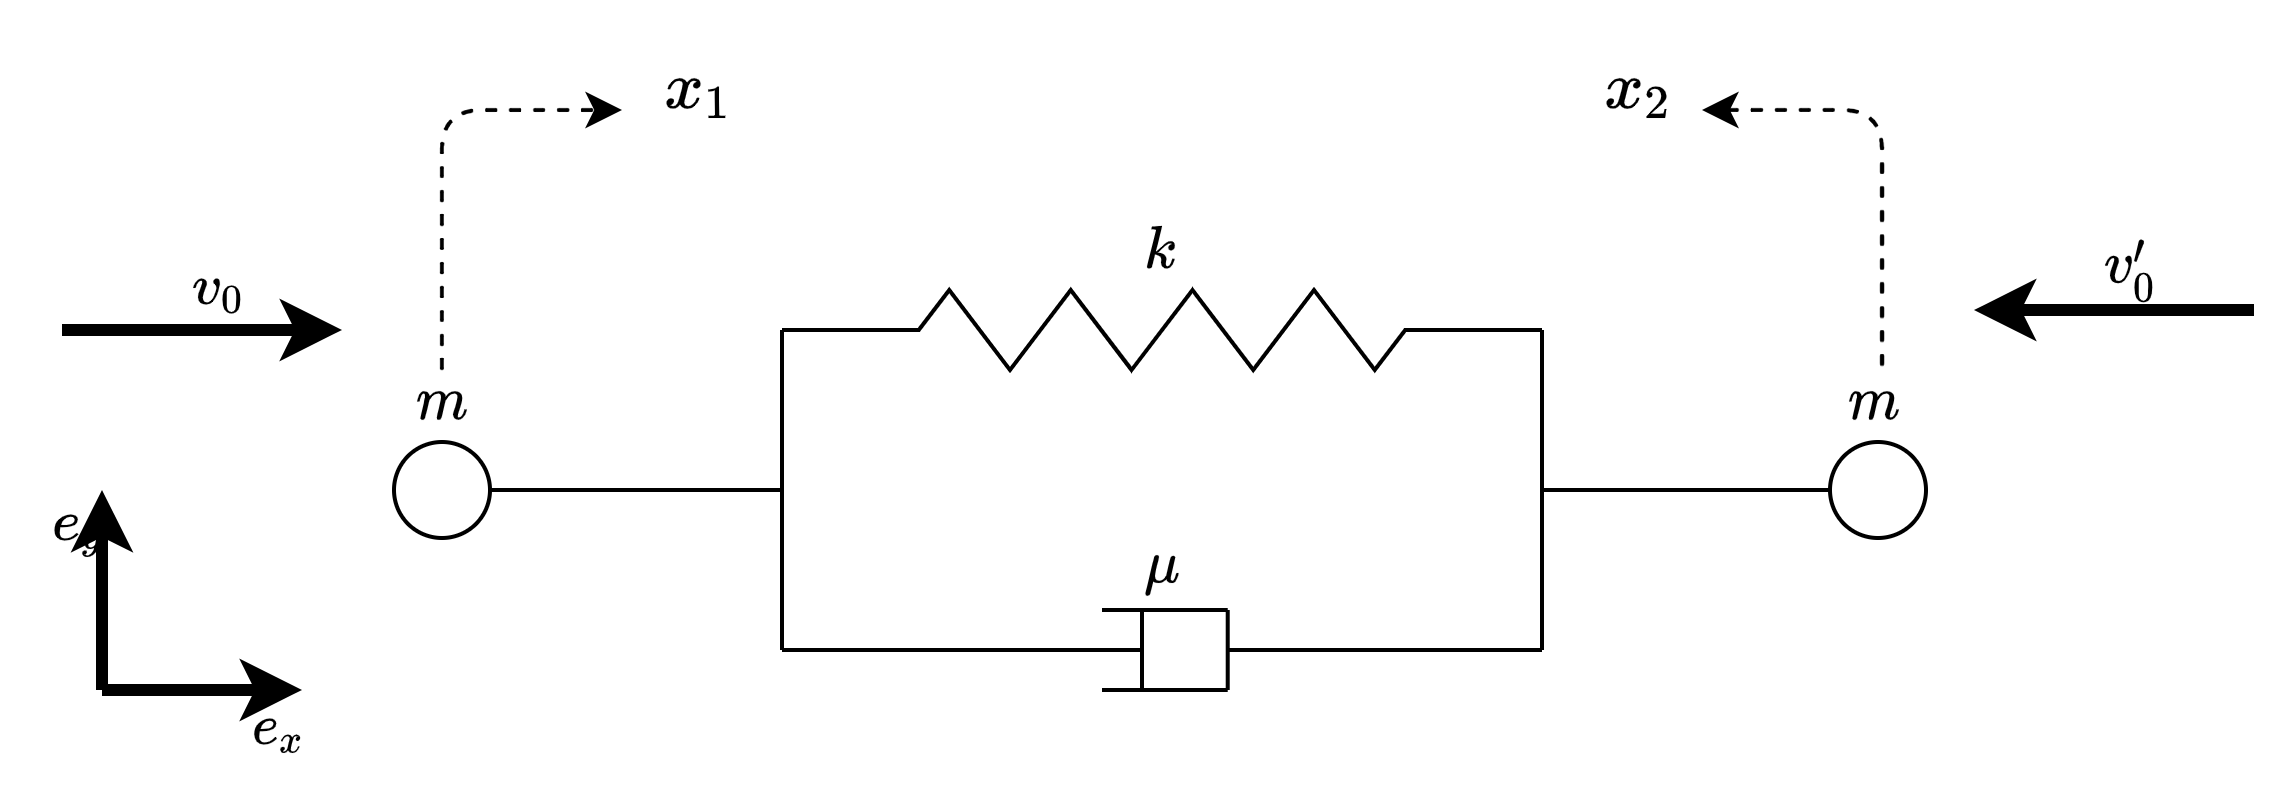
\includegraphics[width=0.6\textwidth]{Deplacement1D-Systeme.png}}
    \caption{Floe de glace 1D modélisé par un réseau de ressorts. Le floe est isolé de toutes forces extérieurs. Les varaibles $x_1$ et $x_2$ traduisent les déplacemnts des noeuds de gauche et de droite respectifs. À l'instant initial, les masses sont soumises aux vitesses $v_0$ et $v'_0$ indiquées.}
    \label{fig:deplacement1d}
\end{figure}


\begin{figure}[!h]
    \begin{subfigure}[b]{0.33\textwidth}
        \centering
        \frame{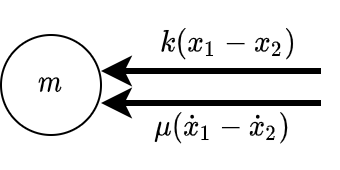
\includegraphics[width=\textwidth]{Deplacement1D-Masse1.png}}
        \caption{Sur la masse $m$ de gauche.}
    \end{subfigure}
%     \hfill
    \begin{subfigure}[b]{0.3\textwidth}
        \centering
        \frame{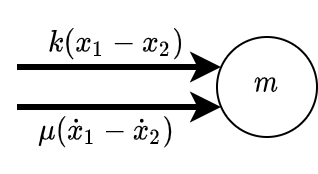
\includegraphics[width=\textwidth]{Deplacement1D-Masse2.png}}
        \caption{Sur la masse $m$ de droite.}
    \end{subfigure}
       \caption{Bilan des forces appliquée sur les noeuds du système. Les valeurs indiquées sont les intensitées (positives) des forces (par exemple juste après l'instant initial, on a $x_1 > 0$, et $x_2 < 0$ d'où $k(x_1-x_2) > 0$).}
       \label{fig:bilan0}
\end{figure}


\noindent Un bilan des forces effectué sur les deux noeuds du floe (voir \cref{fig:bilan0}) permet d'obtenir les équations suivantes:
\begin{align}
    \begin{dcases}
    m\ddot x_1 = - k(x_1 - x_2) - \mu(\dot x_1 - \dot x_2) \,,\\
        m \ddot x_2 =  k(x_1 - x_2) + \mu(\dot x_1 - \dot x_2) \,. 
    \end{dcases}
\end{align}
En remarquant que $m\neq 0$, on passe à la forme matricielle qui s'écrit:
\begin{align}
    \myvec{\ddot{x}_1}{\ddot{x}_2} = 
      \underbrace{ \frac{k}{m} \mymat{-1}{1}{1}{-1}}_{B} \myvec{x_1}{x_2}
    + \underbrace{\frac{\mu}{m} \mymat{-1}{1}{1}{-1}}_{C} \myvec{\dot{x}_1}{\dot{x}_2} \,.
\end{align}
On pose ensuite la matrice par blocs:
\[ E = \mymat{0}{I_2}{B}{C}  =  \begin{pmatrix}
    0 & 0 & 1 & 0 \\ 0 & 0& 0& 1 \\ -\frac{k}{m} & \frac{k}{m} & -\frac{\mu}{m} & \frac{\mu}{m} \\ \frac{k}{m} & -\frac{k}{m} & \frac{\mu}{m} & -\frac{\mu}{m}
\end{pmatrix}   \in \mathbb{R}^{4\times 4} \,, \quad \text{où} \quad I_2 = \mymat{1}{0}{0}{1} \in \mathbb{R}^{2\times 2} \,. \]
On pose maintenant $Y = (x_1, x_2, \dot{x}_1, \dot{x}_2) \in \mathbb{R}^4$, et on reprend la condition initiale pour obtenir le système de Cauchy:
\begin{align} \label{eq:dep1d}
    \begin{dcases}
        \dot{Y}(t)= E Y(t) \,, \\
        Y_0 = Y(t_0) = (0,0,v_0,-v'_0)^T \,.
    \end{dcases}
\end{align}

La solution numérique est présentée dans à la \cref{fig:simudept1d} (voir fichier \verb|code/simu1D/Deplacement1D-1.ipynb| pour plus de détails). La plus grosse remarque à faire du point de vue numérique est que lorsque $v_0 \neq v'_0$, les vitesses convergent vers $0$, mais les déplacements diverge.
\begin{figure*}[!h]
    \centering

    \begin{subfigure}[t]{0.45\textwidth}
        \centering
        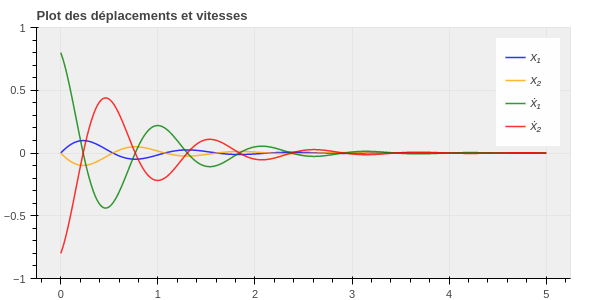
\includegraphics[width=\textwidth]{SimuDeplacement1D1.png}
        \caption{$v_0=v'_0 = 0.8$}
    \end{subfigure}
    \begin{subfigure}[t]{0.45\textwidth}
        \centering
        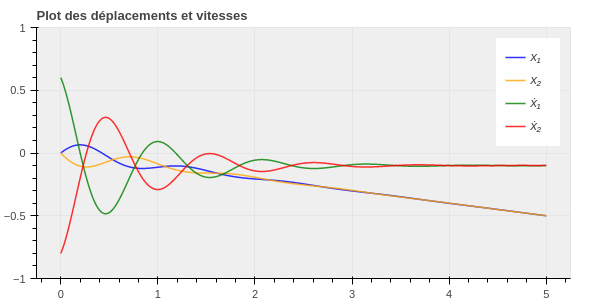
\includegraphics[width=\textwidth]{SimuDeplacement1D2.png}
        \caption{$v_0= 0.6$ et $v'_0 = 0.8$}
    \end{subfigure}

    \caption{Simulation du déplacement 1D d'un floe avec $m=1$, $k=18$, $\mu=1.3$, $t_{f}=5$. En règle générale, on observe le ralentissement du système et une convergence des déplacements vers l'état d'équilibre $Y_{eq}= (0,0,0,0)$ lorsque $v_0 = v'_0$.}
    \label{fig:simudept1d}
\end{figure*}

Avec $t_0= 0$, la solution analytique de ce système d'EDO du premier ordre à coefficients constants est unique et est donnée par.
\begin{align}
    Y(t) = \exp(tE)Y_0 \,.
\end{align}
Nous obtenons le théorème suivant:
\begin{theorem}[Convergence du modèle 1D isolé] \label{th:div1D}
    Partant d'une position d'équilibre $x_1(0) = x_2(0) = 0$, les déplacements $x_1$ et $x_2$ des deux noeuds du floe 1D convergent si et seulement si leurs vitesses initiales sont des vecteurs opposés.
\end{theorem}

\begin{proof}

Le calcul des solution analytique est plus délicat. Il faudrait calculer l'exponentielle de la matrice $E$. Pour celà, nous devons diagonaliser (ou du moins trogonaliser) la matrice $E$. Son polynome caractéristique est donné par:
\begin{align*}    
\text{det}(E-\lambda I_4) &&&= \begin{vmatrix}
    -\lambda & 0 & 1 & 0 \\ 0 & -\lambda & 0& 1 \\ -\frac{k}{m} & \frac{k}{m} & -\frac{\mu}{m}-\lambda & \frac{\mu}{m} \\ \frac{k}{m} & -\frac{k}{m} & \frac{\mu}{m} & -\frac{\mu}{m} -\lambda
\end{vmatrix}, \\
    &&&= \frac{\lambda^2}{m} \left( m\lambda^2 + 2\mu\lambda + 2k \right).
\end{align*}
Posons $\Delta = 4\mu^2 - 8km$. On distingue deux cas:
\begin{itemize}
    \item Si $\Delta \geq 0$: on pose $\lambda_1 = \frac{-\mu - \sqrt{\mu^2 - 2km}}{m}$ et $\lambda_2 = \frac{-\mu + \sqrt{\mu^2 - 2km}}{m}$;
    \item Si $\Delta < 0$: on pose $\lambda_1 = \frac{-\mu - i\sqrt{2km - \mu^2}}{m}$ et $\lambda_2 = \frac{-\mu + i\sqrt{2km - \mu^2}}{m}$.
\end{itemize}
Nous avons donc exhiber les trois valeurs propres de notre matrice: $\lambda_0 = 0$, $\lambda_1$, et $\lambda_2$. Avec $\lambda$ désignant l'une des valeurs propres, on recherche les vecteurs $x = (x_1, x_2, x_3, x_4)^T \in \mathbb{R}^4$ appartenant aux sous espaces propres $E_\lambda$. On a:
\begin{align} \label{eq:espacepropre}
    Ex = \lambda x \Rightarrow \begin{dcases}
        x_3 = \lambda x_1 \\
        x_4 = \lambda x_2 \\
        -(k + \mu \lambda + m \lambda^2) x_1 + (k + \mu \lambda) x_2 = 0 \\
        (k + \mu \lambda) x_1 - (k + \mu \lambda + m \lambda^2) x_2 = 0
    \end{dcases}
\end{align}
\begin{itemize}
    \item Pour $\lambda = 0$, l'\cref{eq:espacepropre} revient à:
    \begin{align*}
        \begin{dcases}            
        x_3 = 0 \\
        x_4 = 0 \\
        x_1 - x_2 = 0
        \end{dcases}
    \end{align*} 
    On en déduit $E_0 = \text{vect}\{ e_1 \}$, avec $e_1 = (1,1,0,0)^T$.
    \item Pour $\lambda = \lambda_1, \lambda_2$, on remarque que $k + \mu \lambda + m \lambda^2 = - (k + \mu \lambda)$. l'\cref{eq:espacepropre} revient donc à:
    \begin{align*}
        \begin{dcases}            
        x_3 = \lambda x_1 \\
        x_4 = \lambda x_2 \\
        x_1 + x_2 = 0
        \end{dcases}
    \end{align*} 
    On en déduit donc $E_{\lambda_1} = \text{vect}\{ e_3 \}$, avec $e_3 = (1,-1,\lambda_1,-\lambda_1)^T$; et $E_{\lambda_2} = \text{vect}\{ e_4 \}$ avec $e_4 = (1,-1,\lambda_2,-\lambda_2)^T$.
\end{itemize}
La meutilisicté arithmetique de $\lambda = 0$ est differente de sa multiplicité géometrique. La matrice $E$ n'est donc pas diagonalisable. Son polynome caractéristique étant scindé, nous alons la trigonaliser. On pose donc une base $\mathcal{B}' = (v_1, v_2, v_3, v_4)$ dans laquelle la matrice $E$ s'exprime par:
\begin{align*}
    P^{-1}EP = \begin{pmatrix}
        0 & a & b & c \\ 0 & 0 & d & e \\ 0 & 0 & \lambda_1 & f \\ 0 & 0 & 0 & \lambda_2
    \end{pmatrix},
\end{align*}
où $P$ est la matrice de passage de la base canonique de $\mathbb{R}^4$ (notée $\mathcal{B}$) à $\mathcal{B}'$. On a:
\begin{itemize}
    \item Dans $\mathcal{B}'$, le vecteur $v_1$ s'écrit $v_1 = (1,0,0,0)^T$ et on a $P^{-1}EP v_1 = 0$. $v_1$ est donc le vecteur propre associé à $0$ et on prend $v_1 = e_1 = (1,1,0,0)^T$ dans $\mathcal{B}$;
    \item Dans $\mathcal{B}'$, le vecteur $v_2$ s'écrit $v_2 = (0,1,0,0)^T$ et on a $P^{-1}EP v_2 = a v_1$. On retourne dans $\mathcal{B}$ en posant $v_2 = (x_1, x_2, x_3, x_4)^T$ pour obtenir le système:
    \begin{align*}
        E v_2 = a v_1 \Rightarrow
        \begin{dcases}            
        x_3 = a  \\
        x_4 = a  \\
        x_1 - x_2 = 0
        \end{dcases}.
    \end{align*} 
    Avec $a = 1$, on écrit $v_2 = e_2 = (1,1,1,1)^T$.
    \item Dans $\mathcal{B}'$, le vecteur $v_3$ s'écrit $v_1 = (0,0,1,0)^T$ et on a $P^{-1}EP v_1 = \lambda_1 v_1 + bv_1 + d v_2$. En posant $b=d=0$, $v_1$ devient un vecteur propre associé à $\lambda_1$ et on prend $v_3 = e_3 = (1,-1,\lambda_1,-\lambda_1)^T$ dans $\mathcal{B}$;
    \item De facon similaire, on obtient $v_4 = e_4 = (1,-1,\lambda_2,-\lambda_2)^T$ en posant $c=e=f=0$.
\end{itemize}
Nous avons donc trigonaliser la matrice $E$, et on écrit :
\begin{align*}
    P^{-1}EP = A, \text{avec} A = \begin{pmatrix}
        0 & 1 & 0 & 0 \\ 0 & 0 & 0 & 0 \\ 0 & 0 & \lambda_1 & 0 \\ 0 & 0 & 0 & \lambda_2
    \end{pmatrix}, \text{  } P = \begin{pmatrix}
        1 & 1 & 1 & 1 \\ 1 & 1 & -1 & -1 \\ 0 & 1 & \lambda_1 & \lambda_2 \\ 0 & 1 & -\lambda_1 & -\lambda_2
    \end{pmatrix}, \text{ et } P^{-1} = \frac{1}{2}\begin{pmatrix}
        1 & 1 & -1 & -1 \\ 0 & 0 & 1 & 1 \\ \frac{\lambda_2}{\lambda_2-\lambda_1} & -\frac{\lambda_2}{\lambda_2-\lambda_1} & -\frac{1}{\lambda_2-\lambda_1} & \frac{1}{\lambda_2-\lambda_1} \\ -\frac{\lambda_1}{\lambda_2-\lambda_1} & \frac{\lambda_1}{\lambda_2-\lambda_1} & \frac{1}{\lambda_2-\lambda_1} & -\frac{1}{\lambda_2-\lambda_1}
    \end{pmatrix}.
\end{align*}
La matrice $A$ se décompose en somme d'une matrice diagonale et d'une matrice nilpotente $A = D+N$ avec:
\begin{align*}
    D = \begin{pmatrix}
        0 & 0 & 0 & 0 \\ 0 & 0 & 0 & 0 \\ 0 & 0 & \lambda_1 & 0 \\ 0 & 0 & 0 & \lambda_2
    \end{pmatrix}, \text{ et } N = \begin{pmatrix}
        0 & 1 & 0 & 0 \\ 0 & 0 & 0 & 0 \\ 0 & 0 & 0 & 0 \\ 0 & 0 & 0 & 0
    \end{pmatrix}.
\end{align*}
En posant $E = P(D+N)P^{-1}$, nous pouvons facilemtn calculer $\forall t \in \mathbb{R}$, $\exp(tE) = P\exp(tD)\exp(tN)P^{-1}$. Ce calcul délicat donne (à l'aide du logiciel de calcul symbolique $\verb|Symbolab|$):
\begin{align*}
    \exp(tE) = \tiny \frac{1}{2(\lambda_2 - \lambda_1)}\begin{pmatrix} 
        \lambda_2e^{t\lambda_1} + \lambda_2 - \lambda_1 - \lambda_1e^{t\lambda_2} & -\lambda_2e^{t\lambda_1} + \lambda_2 - \lambda_1 + \lambda_1e^{t\lambda_2} & t(\lambda_2 -\lambda_1) - e^{t\lambda_1} + e^{t\lambda_2} & t(\lambda_2 -\lambda_1) + e^{t\lambda_1} - e^{t\lambda_2} \\
         -\lambda_2e^{t\lambda_1} + \lambda_2 - \lambda_1 + \lambda_1e^{t\lambda_2} & \lambda_2e^{t\lambda_1} + \lambda_2 - \lambda_1 - \lambda_1e^{t\lambda_2} & t(\lambda_2 -\lambda_1) + e^{t\lambda_1} - e^{t\lambda_2} & t(\lambda_2 -\lambda_1) - e^{t\lambda_1} + e^{t\lambda_2} \\
          \lambda_1\lambda_2 (e^{t\lambda_1} - e^{t\lambda_2}) & \lambda_1\lambda_2 (e^{t\lambda_2} - e^{t\lambda_1})  & -\lambda_1e^{t\lambda_1} + \lambda_2 - \lambda_1 + \lambda_2e^{t\lambda_2} & \lambda_1e^{t\lambda_1} + \lambda_2 - \lambda_1 - \lambda_2e^{t\lambda_2} \\
          \lambda_1\lambda_2 (e^{t\lambda_2} - e^{t\lambda_1})  & \lambda_1\lambda_2 (e^{t\lambda_1} - e^{t\lambda_2})  & \lambda_1e^{t\lambda_1} + \lambda_2 - \lambda_1 - \lambda_2e^{t\lambda_2} & -\lambda_1e^{t\lambda_1} + \lambda_2 - \lambda_1 + \lambda_2e^{t\lambda_2}
    \end{pmatrix}.
\end{align*}
Rappelons nous que la solution du problème de Cauchy \cref{eq:dep1d} est donnée par $Y(t) = \exp(tE)Y_0$, avec $Y_0 = (0,0,v_0,-v'_0)$. Le calcul du déplacement $x_1$ donne:
\begin{align} \label{eq:solreel}
    x_1(t) = \frac{t}{2}\left( v_0 - v'_0 \right) - \frac{e^{t\lambda_1} - e^{t\lambda_2}}{2(\lambda_2 - \lambda_1)}\left( v_0 + v'_0 \right).
\end{align}
Le cas où $\Delta < 0$ (à étudier dans $\mathbb{C}$) peut se ramener au cas réel (dans $\mathbb{R}$) en posant $\lambda_1 = \alpha + i \beta$ et $\lambda_2 = \alpha - i \beta = \bar{\lambda}_1$ (avec $\alpha = -\frac{\mu}{m}$ et $\beta = -\frac{\sqrt{2km - \mu^2}}{m}$). En remarquant que $\sin(\beta t) = \frac{e^{i\beta t} - e^{-i\beta t}}{2i}$, on obtient :
\begin{align} \label{eq:solcomplexe}
    x_1(t) = \frac{t}{2}\left( v_0 - v'_0 \right) + \frac{e^{\alpha t} \sin(\beta t)}{2\beta} \left( v_0 + v'_0 \right).
\end{align}
Les \cref{eq:solreel,eq:solcomplexe} permettent d'observer que le déplacement $x_1$ ne converge pas lorsque $t \rightarrow +\infty$, à moins que $v_0 = v'_0$, ce qui est observé à la \cref{fig:simudept1d}. Pour le déplacement du deuxième noeud, on a:
\begin{align} \label{eq:solcomplexe}
    x_2(t) = \frac{t}{2}\left( v_0 - v'_0 \right) - \frac{e^{\alpha t} \sin(\beta t)}{2\beta} \left( v_0 + v'_0 \right);
\end{align}
On tire les mêmes conclusions en effectuant un raisonnement similaire.

\end{proof}










%2----------------------------------------------------------------------------------------



\section{Modélisation de la percussion}









\subsection{Collision parfaitement inélastique avec un floe encastré à l'instant initial}



Nous effectuons ici une modélisation 1D de notre problème de percussion. Un floe est modélisé par un système masse-ressort de deux noeuds. Le floe 1 est immobilisé face au mur, et le floe 2 approche à la vitesse $\bvec{v}_0$. On identifie chaque noeud à la masse qu'il porte ($m$ ou $m'$), chaque ressort à sa raideur ($k$ ou $k'$), chaque dispositif visqueux à sa viscosité ($\mu$ ou $\mu'$) (voir \cref{fig:contact1d}).
\begin{figure}[!h]
    \centering
    \frame{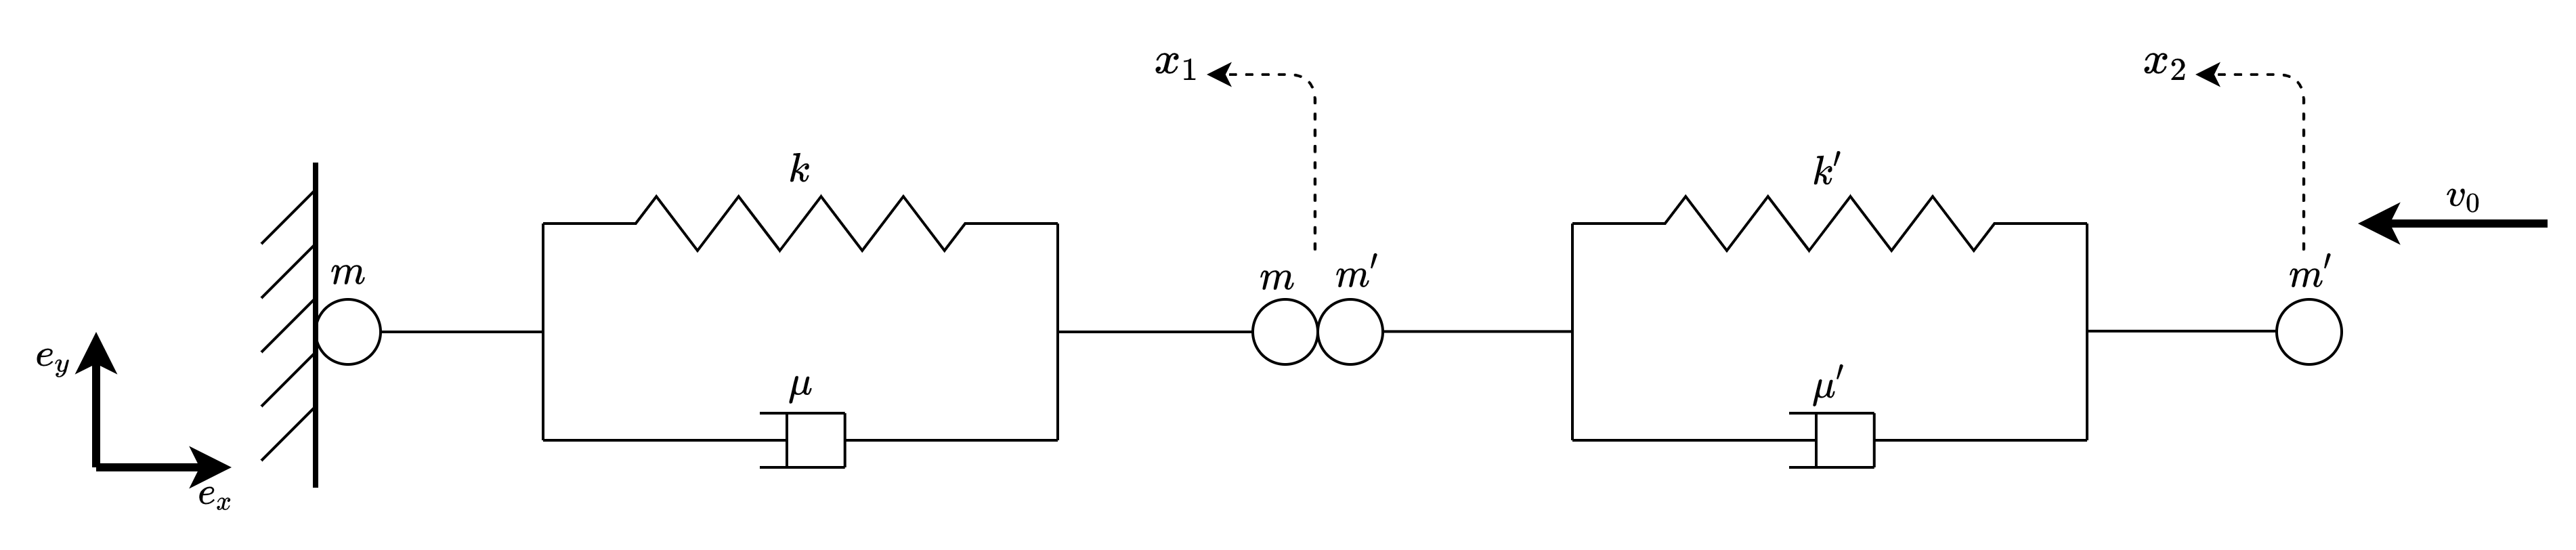
\includegraphics[width=0.8\textwidth]{Percussion1D-Systeme}}
    \caption{Contact 1D parfaitement inélastique (choc mou) entre deux floes. Le floe percuté étant immobile et coincé au mur avant, durant, et après le choc.}
    \label{fig:contact1d}
\end{figure}

\noindent On suppose que durant la dynamique non régulière, les masses $m$ et $m'$ en contact forment une seule masse\footnote{Cette simplification a pour principal avantage de supprimer le traitement de la force de contact entre les deux masses.}
$m+m'$ dont
le déplacement est donné par la variable $x_1(t)$. Le déplacement de la masse $m'$ à l'autre bout du floe percuteur est nommé
$x_2(t)$. La masse $m$ qui est fixée au mur ne sera pas étudiée ici. Nous faisons à présent le bilan des forces qui
s'exercent ces
deux masses.
\begin{figure}[!h]
     \begin{subfigure}[b]{0.4\textwidth}
         \centering
         \frame{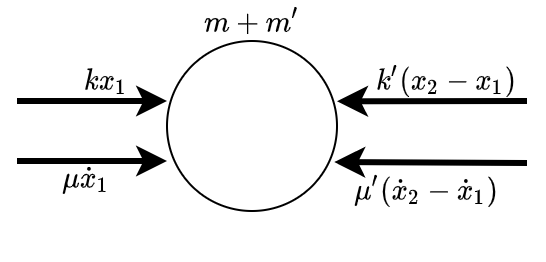
\includegraphics[width=\textwidth]{Percussion1D-Masse1}}
         \caption{Sur $m+m'$.}
         \label{fig:bilan11}
     \end{subfigure}
%     \hfill
     \begin{subfigure}[b]{0.3\textwidth}
         \centering
         \frame{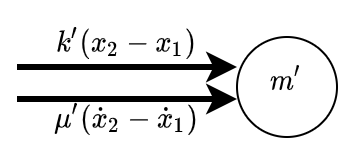
\includegraphics[width=\textwidth]{Percussion1D-Masse2}}
         \caption{Sur $m'$.}
         \label{fig:bilan12}
     \end{subfigure}
        \caption{Bilan des forces appliquée sur les noeuds du système. Les valeurs indiquées sont les intensitées
            (positives) des forces durant une phase imaginée de compression des ressorts ($\bvec{v}_0 <0$ et donc
            $x_1 <0$). Pour obtenir l'intesité de la force de rappel du ressort $k'$, on peut imaginer $x_1$ imobile
            (on aura $x_2 < 0$, d'où $x_1 - x_2 > 0$) (voir \parencite{homodeling}).}
        \label{fig:bilan}
\end{figure}

\noindent En orientant convenablement le système (voir \cref{fig:contact1d}), on applique la loi de Newton-Euler linéaire
pour obtenir le système suivant et ses conditions initiales \footnote{J'ai des doutes sur cette condition
initiale. La vitesse initiale de $x_1$ est-elle vraiment nulle?}:
\begin{align}
    \begin{dcases}
    (m+m')\ddot x_1 = -kx_1 - \mu \dot x_1 + k'(x_2 - x_1) + \mu'(\dot x_2 - \dot x_1) \\
        m' \ddot x_2 =  -k'(x_2 - x_1) - \mu'(\dot x_2 - \dot x_1) 
    \end{dcases}
\end{align}
À l'instant initial $t_0$, on a le système suivant
\begin{align} \label{eq:percussion1d}
    \begin{dcases}
    (x_1(t_0), x_2(t_0)) = (0,0) \\
    (\dot x_1(t_0), \dot x_2(t_0)) = (0,-v_0)
    \end{dcases}
\end{align}
En posant $X = (x_1, x_2)^T \in \mathbb{R}^2$, l' \cref{eq:percussion1d} devient
\begin{align}
    \underbrace{\mymat{m+m'}{0}{0}{m'}}_{A} \myvec{\ddot{x}_1}{\ddot{x}_2} = \underbrace{\mymat{-k-k'}{k'}{k'}{-k'}}_{B} \myvec{x_1}{x_2} + \underbrace{\mymat{-\mu -\mu^\prime}{\mu'}{\mu'}{-\mu'}}_{C} \myvec{\dot{x}_1}{\dot{x}_2} \,.
\end{align}
Puisque $m, m'\neq 0$, la matrice $A$ est inversible et on obtient au final le problème de Cauchy suivant:
\begin{align} \label{eq:percussion1d2}
    \begin{dcases}
        \ddot{X}(t) = B' \dot{X}(t) + C'X(t) \,, \\
        (X(t_0), \dot X (t_0)) = \left( \myvec{0}{0}, \myvec{0}{-v_0} \right) \,,
    \end{dcases}
\end{align}
avec $B' = A^{-1}B$ et $C' = A^{-1}C$.

\noindent Il s'agit la d'un système d'EDO du deuxième ordre à coefficients constants. Transformons le en un système du premier ordre pour
une résolution plus aisée. On pose donc $Y= (X, \dot X)^T = (x_1, x_2, \dot{x}_1, \dot{x}_2)^T \in \mathbb{R}^4$ et le
système
\ref{eq:percussion1d2}
devient
\begin{align} \label{eq:systeme1d}
    \begin{dcases}
        \dot{Y}(t)= E Y(t) \\
        Y_0 = Y(t_0) = (0,0,0,-v_0)^T
    \end{dcases}
\end{align}
avec la matrice par blocs \[ E = \mymat{0}{I_2}{B'}{C'} \,, \] où $I_2$ désigne la matrice identité de
$\mathbb{R}^{2\times2}$.

\noindent Avec $t_0= 0$, la solution de ce système d'EDO du premier ordre à coefficients constants est unique et est donnée par
\begin{align}
    Y(t) = \exp(tE)Y_0
\end{align}

La résolution analytique du système passe par le calcul de l'exponentielle de la matrice $E \in \mathbb{R}^4$, ce qui s'avère difficile du à la taille de ladite matrice. Nous optons donc pour une solution numérique (voir figure \cref{fig:simucontact1dun}) issue du notebook $\verb|code/simu1D/Percussion1D-1.ipynb|$.
% \begin{figure}[!h]
%     \centering
%     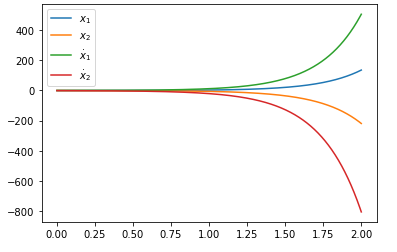
\includegraphics[width=0.4\textwidth]{SimuPercussion1D.png}
%     \caption{Simulation de la percussion 1D entre deux floes avec $m=1$, $m'=1$, $k=16$, $k'=5$, $\mu=6$,
%         $\mu'=2$, $v_0=-1.0$, $t_{f}=32$. On observe effectivement le ralentissement du système et une convergence
%         vers l'état d'équilibre $Y_{eq}= (0,0,0,0)$.}
%     \label{fig:simucontact1d}
% \end{figure}
\begin{figure*}[!h]
    \centering

    \begin{subfigure}[t]{0.48\textwidth}
        \centering
        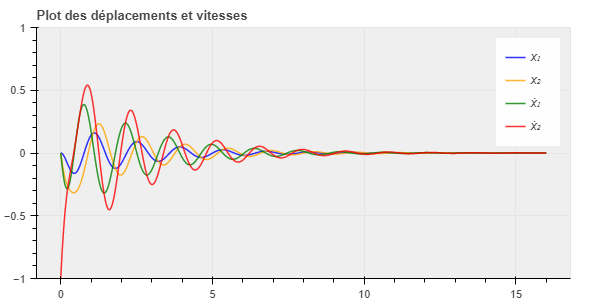
\includegraphics[width=\textwidth]{SimuPercussion1D-1.png}
        \caption{$\mu= 4.0$ et $\mu' = 2.5$ }
        \label{fig:simucontact1dun}
    \end{subfigure}
    \begin{subfigure}[t]{0.48\textwidth}
        \centering
        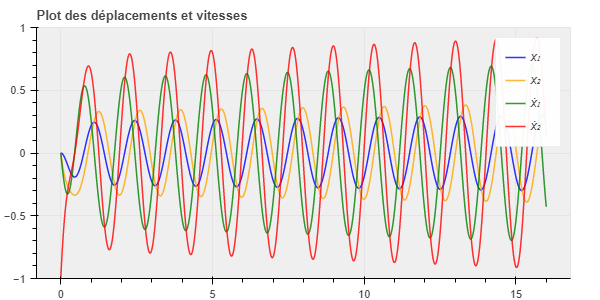
\includegraphics[width=\textwidth]{SimuPercussion1D-2.png}
        \caption{$\mu= 2.8$ et $\mu' = 2.5$ }
        \label{fig:simucontact1ddeux}
    \end{subfigure}
    \caption{Simulation de la percussion 1D entre deux floes avec $m=1$, $m'=1$, $k=16$, $k'=5$, $v_0=-1.0$, $t_{f}=32$. Dans le premier cas (a), on observe effectivement le ralentissement du système et une convergence
    vers l'état d'équilibre $Y_{eq}= (0,0,0,0)$. Dans le second cas (b), on constate que le système diverge.}
    \label{fig:simucontact1d}
\end{figure*}




\noindent Pour certaines valeurs (specifiquement de $\mu$ et $\mu'$), on constate que le système converge vers son état d'équilibre attendu $Y_{eq} = (0,0,0,0)$. En revanche pour certaines (voir \cref{fig:simucontact1ddeux}), il diverge\footnote{La divergence pour ce cas est particulièrement évidente lorsque $\mu < \mu'$.}. Pour étendre les travaux dans cette section, on pourrait:
\begin{enumerate}
    \item Calculer analytiquement et numériquement les état d'équilibres $Y_{eq} \in \ker(E)$; puis en distinguer les états stables des autres.
    \item Calculer analytiquement l'exponentielle de la matrice $E$, et donner l'expression de la solution; déduire la condition sur les parametres pour que le système converge vers l'état d'équilibre voulu.
\end{enumerate} 








\subsection{Collision parfaitement inélastique sans présence du mur}

Contrairement au cas étudié dans la section précédente, le mur est supprimé ici. On ajoute donc une troisième variable afin de décrire le comportement du noeud qui était rattaché au mur. La schéma régissant ce système est donnée à la \cref{fig:contact1d2}. Le bilan des forces appliquées aux noeuds est présenté à la \cref{fig:bilan2}.

\begin{figure}[!h]
    \centering
    \frame{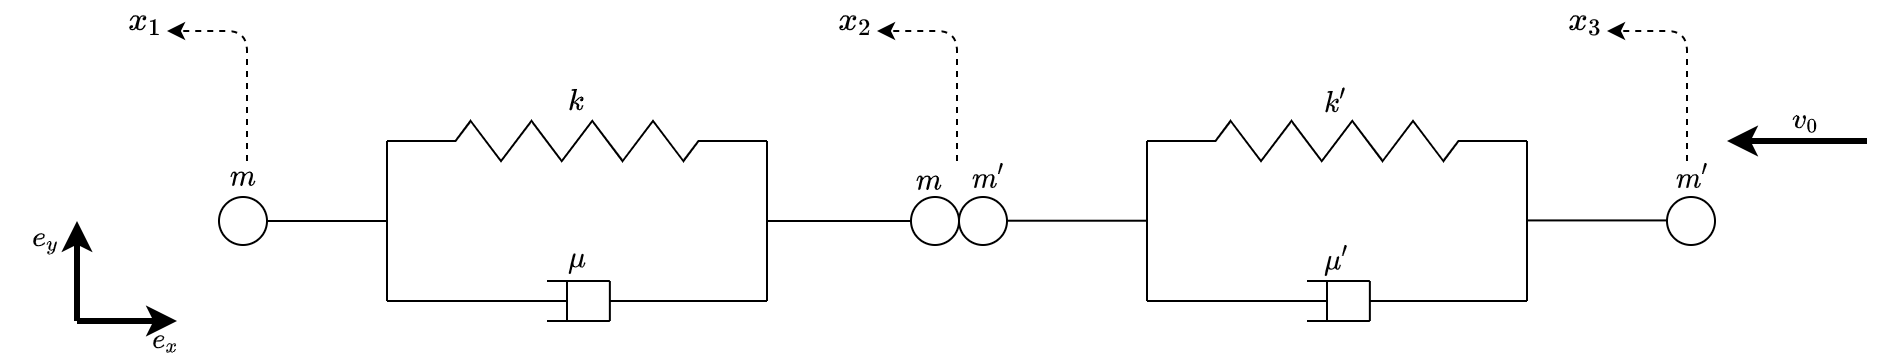
\includegraphics[width=0.8\textwidth]{Percussion1D-Systeme-2}}
    \caption{Contact 1D parfaitement inélastique entre deux floes. Le floe percuté étant non immobile (et non coincé au mur) avant le choc. On représnte également les variables $x_1$, $x_2$, et $x_3$ décrivant les movements de chaque noeud.}
    \label{fig:contact1d2}
\end{figure}

\begin{figure}[!h]
    \begin{subfigure}[b]{0.25\textwidth}
        \centering
        \frame{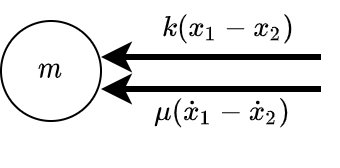
\includegraphics[width=\textwidth]{Percussion1D2-Masse1.png}}
        \caption{Sur $m$.}
        \label{fig:bilan12}
    \end{subfigure}
%     \hfill
    \begin{subfigure}[b]{0.31\textwidth}
        \centering
        \frame{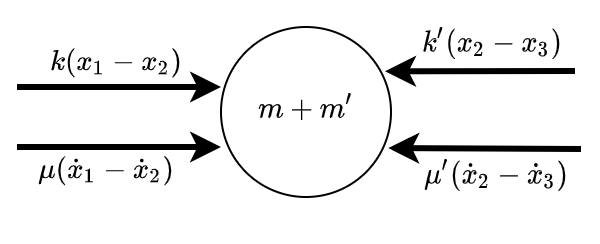
\includegraphics[width=\textwidth]{Percussion1D2-Masse2}}
        \caption{Sur $m+m'$.}
        \label{fig:bilan22}
    \end{subfigure}
%     \hfill
    \begin{subfigure}[b]{0.23\textwidth}
        \centering
        \frame{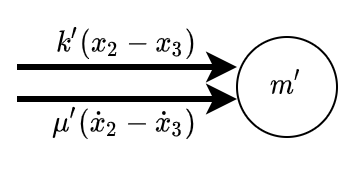
\includegraphics[width=\textwidth]{Percussion1D2-Masse3}}
        \caption{Sur $m'$.}
        \label{fig:bilan32}
    \end{subfigure}
       \caption{Bilan des forces appliquée sur les noeuds du système. On procède de facon similaire à \cref{fig:bilan} pour obtenir les sens et les intensités de ces forces.}
       \label{fig:bilan2}
\end{figure}

\noindent Comme précédement, nous appliqons les lois de Newton pour obtenir:
\begin{align}
    \begin{dcases}
    m\ddot x_1 = -k(x_1 - x_2) - \mu (\dot x_1 - \dot x_2) \,, \\
    (m+m')\ddot x_2 = k(x_1 - x_2) + \mu (\dot x_1 - \dot x_2) - k'(x_2 - x_3) - \mu'(\dot x_2 - \dot x_3) \,, \\
        m' \ddot x_3 =  k'(x_2 - x_3) + \mu'(\dot x_2 - \dot x_3) \,. 
    \end{dcases}
\end{align}
Sous forme matricielle, on a
\begin{align}
    \underbrace{\mybigmat{m}{0}{0}{0}{m+m'}{0}{0}{0}{m'}}_{A} \mybigvec{\ddot{x}_1}{\ddot{x}_2}{\ddot{x}_3} =  
    \underbrace{\mybigmat{-k}{k}{0}{k}{-k-k'}{k}{0}{k'}{-k'}}_{B} \mybigvec{x_1}{x_2}{x_3} + 
    \underbrace{\mybigmat{-\mu}{\mu}{0}{\mu}{-\mu-\mu'}{\mu'}{0}{\mu'}{-\mu'}}_{C} \mybigvec{\dot{x}_1}{\dot{x}_2}{\dot{x}_3} \,.
\end{align}
Puisque $m, m'\neq 0$, la matrice $A$ est inversible. En posant $X = (x_1, x_2, x_3)^T \in \mathbb{R}^3$, le système d'EDO revient à l' \cref{eq:percussion1d22} suivante:
\begin{align} \label{eq:percussion1d22}
        \ddot{X}(t) = B' X(t) + C'\dot{X}(t) \,, 
\end{align}
où $B' = A^{-1}B$ et $C' = A^{-1}C$. On pose ensuite $Y= (X, \dot X)^T \in \mathbb{R}^6$ et le système \cref{eq:percussion1d22} devient 
\begin{align} \label{eq:systeme1d2}
        \dot{Y}(t)= E Y(t)
\end{align}
avec $$ E = \mymat{0}{I_3}{B'}{C'} \,.$$


Remarquons qu'en enlevant le mur à gauche du domaine (voir \cref{fig:contact1d}), le système est devenu isolé. Nous pouvons donc appliquer la conservation de la quantité de mouvement pour identifier la vitesse de l'ensemble de masse $2(m+m')$ après collision et fixation de la masse $m'$ (à vitesse $\bvec{v}_0$) sur la masse $m$ (de vitesse $\bvec{v}'_0$)\footnote{Le vecteur $\bvec{v}'_0$ n'est pas marqué à la \cref{fig:contact1d2} (i.e. $\bvec{v}'_0 = 0$). L'introduction de ce vecteur permet de généraliser le problème.}. Pour simplifier les calculs, nous considérons les floes comme des solides rigides. La vitesse de l'ensemble juste après collision est notée $v_f$, et les quantités de mouvement avant et après choc sont notées $P_{\text{avant}}$ et $P_{\text{après}}$. On a :
\begin{align*}
    & \quad P_{\text{avant}} = P_{\text{après}} \\
    \Rightarrow & \quad 2m \bvec{v}_0 + 2m'\bvec{v'}_0 = (2m + 2m') \bvec{v}_f \\
    \Rightarrow & \quad \bvec{v}_f = \frac{m \bvec{v}_0 + m'\bvec{v'}_0}{m+m'}
\end{align*} 

\noindent On introduit ces conditions initiales dans l'\cref{eq:systeme1d2} pour obtenir le système de Cauchy ci-bas. Le résulat de la simulation est présenté à la figure \cref{fig:simucontact1d2} (issue du notebook $\verb|code/simu1D/Percussion1D-2.ipynb|$). 
\begin{align} \label{eq:systeme1d3}
    \begin{dcases}
        \dot{Y}(t)= E Y(t) \,, \\
        Y(t_0) = Y_0 = -v_f(0,0,0,1,1,1) \,.        
    \end{dcases}
\end{align}

\begin{figure}[!h]
    \centering
    \begin{subfigure}{0.45\textwidth}
        \centering
        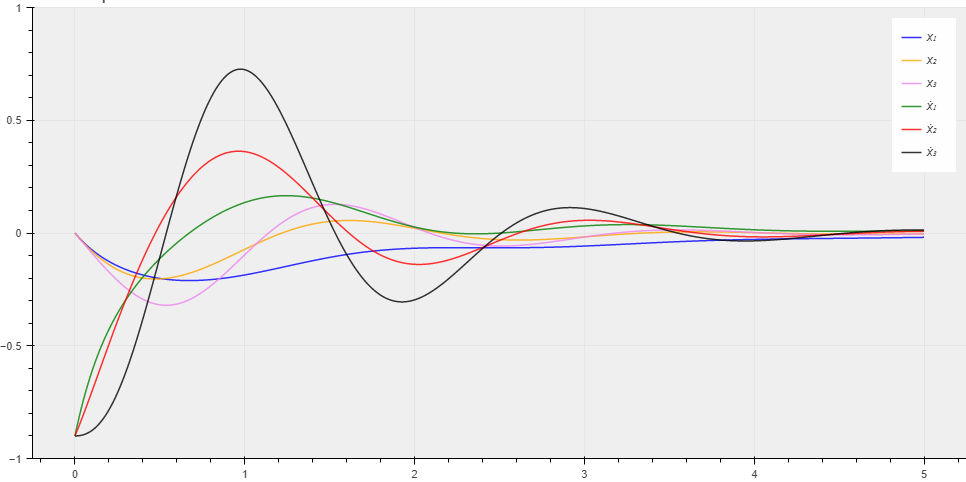
\includegraphics[width=\textwidth]{SimuPercussion1D2.png}
        \caption{$k=3$}
    \end{subfigure}
    \begin{subfigure}{0.45\textwidth}
        \centering
        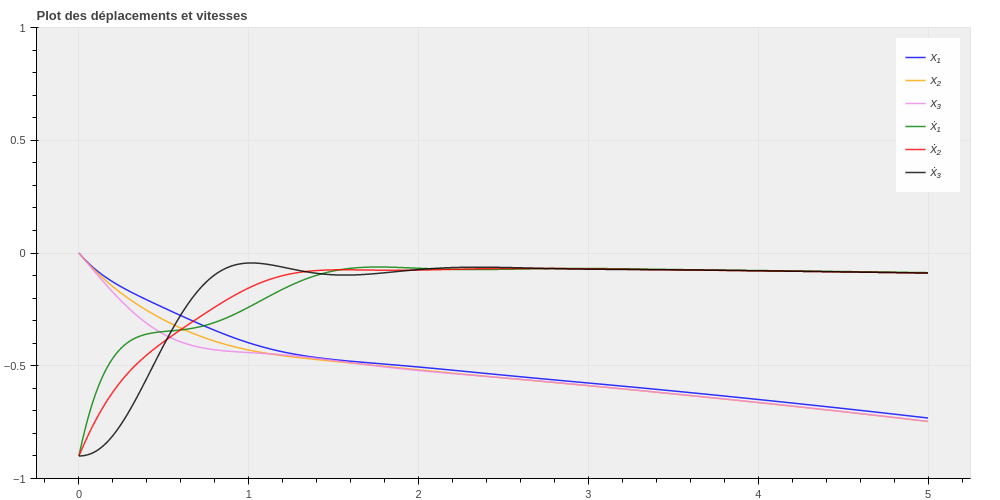
\includegraphics[width=\textwidth]{SimuPercussion1D2NonConv.png}
        \caption{$k=23$}
    \end{subfigure}

    \caption{Simulation de la percussion 1D entre deux floes (sans présence du mur) avec $m=1$, $m'=1$, $k'=22$, $\mu=6$, $\mu'=2$, $v_0=-1.8$, $t_{f}=5$. Sous certaines conditions (forte dissipation, raideur du floe percuté élevée, etc.), on observe le ralentissement du système et une convergence vers l'état d'équilibre $Y_{eq}=(0,0,0,0,0,0)$.} 
    \label{fig:simucontact1d2}
\end{figure}

\noindent La \cref{fig:simucontact1d2} permet d'observer la nuance avec le problème de contact parfaitemetn inélastique. Il est difficile de distinguer les cas qui aboutissent à une convergences des déplacements de ceux qui divergent. Observons donc à présent un problème de contact inélastique avec séparation des masses.






\subsection{Premier modèle pour la collision inélastique avec séparation des masses}
\label{subsubsec:colinesepma}

Reprennons le cas du contact 1D et étudions ce qui se passe durant l'intervale de temps $\tdelta = [\tmoins, \tplus]$ de la collision. Cette fois, pour étudier la dynamique non régulière, nous décidons de séparer les masses $m$ et $m'$ en contact (et ce même durant le contact). Le système résultant est très similaire aux deux cas traités précédemment (\cref{fig:contact1d,fig:contact1d2}), et nous le présentons à la \cref{fig:contact1d3} ci-bas, et son bilan de forces à la \cref{fig:bilan3}.

\begin{figure}[!h]
    \centering
    \frame{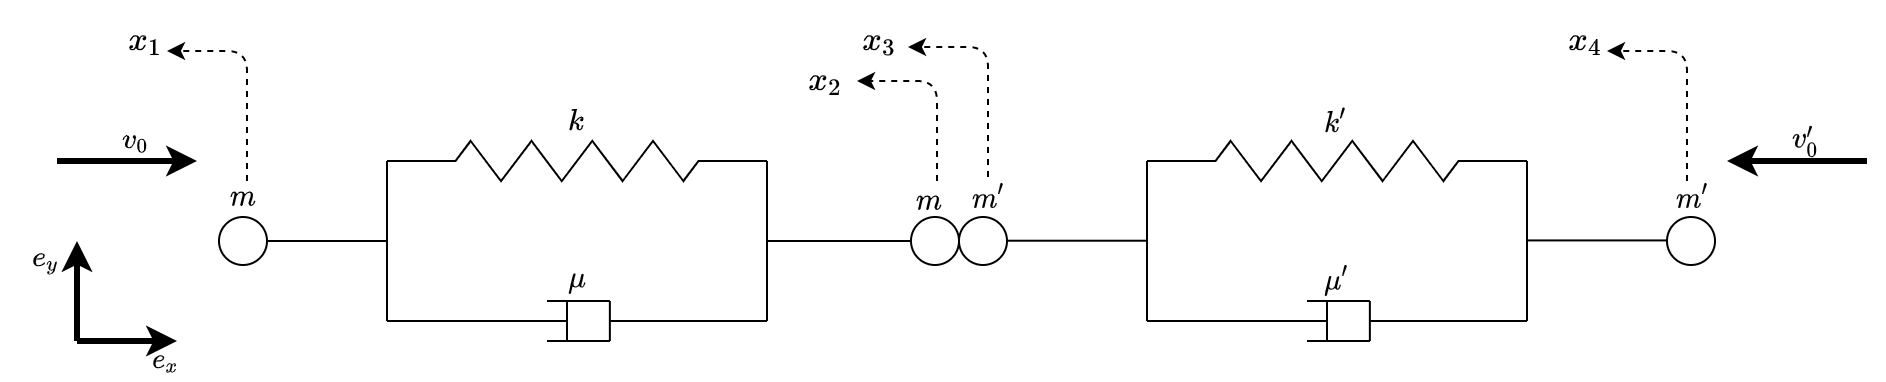
\includegraphics[width=0.8\textwidth]{Percussion1D-Systeme-3}}
    \caption{Contact 1D inélastique entre deux floes. Durant le choc, les nœuds $m$ et $m'$ en contact sont étudiés séparement. On représnte les variables $x_1$, $x_2$, $x_3$, et $x_4$ décrivant les movements de chaque noeud.}
    \label{fig:contact1d3}
\end{figure}


\begin{figure}[!h]
    \begin{subfigure}[b]{0.30\textwidth}
        \centering
        \frame{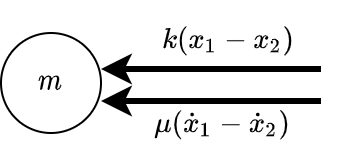
\includegraphics[width=\textwidth]{Percussion1D3-Masse1.png}}
        \caption{Sur $m$ de gauche ($x_1$).}
        \label{fig:bilan13}
    \end{subfigure}
%     \hfill
    \begin{subfigure}[b]{0.42\textwidth}
        \centering
        \frame{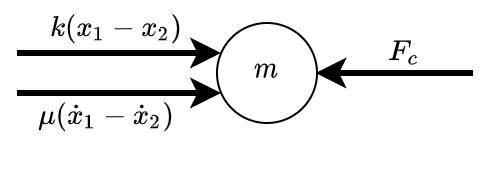
\includegraphics[width=\textwidth]{Percussion1D3-Masse2}}
        \caption{Sur $m$ de droite ($x_2$).}
        \label{fig:bilan23}
    \end{subfigure}
%     \hfill
    \begin{subfigure}[b]{0.423\textwidth}
        \centering
        \frame{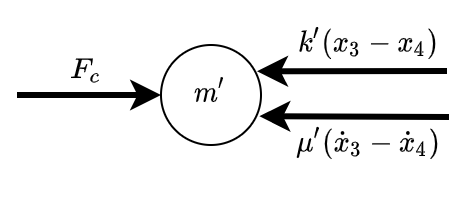
\includegraphics[width=\textwidth]{Percussion1D3-Masse3}}
        \caption{Sur $m'$ de gauche ($x_3$).}
        \label{fig:bilan33}
    \end{subfigure}
%     \hfill
    \begin{subfigure}[b]{0.297\textwidth}
        \centering
        \frame{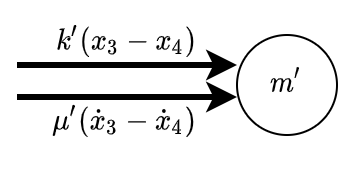
\includegraphics[width=\textwidth]{Percussion1D3-Masse4}}
        \caption{Sur $m'$ de droite ($x_4$).}
        \label{fig:bilan43}
    \end{subfigure}
       \caption{Bilan des forces appliquée sur les $4$ noeuds du système. On procède de facon similaire aux \cref{fig:bilan,fig:bilan2} pour obtenir les sens et les intensités de ces forces. $F_c$ représente la force de contact dont l'intensité est inconnue.}
       \label{fig:bilan3}
\end{figure}

\noindent Comme précédement, nous appliqons les lois de Newton pour obtenir:
\begin{align}
    \begin{dcases}
    m\ddot x_1 = -k(x_1 - x_2) - \mu (\dot x_1 - \dot x_2) \,, \\
    m\ddot x_2 = k(x_1 - x_2) + \mu (\dot x_1 - \dot x_2) - F_c \,, \\
    m'\ddot x_3 = - k'(x_3 - x_4) - \mu'(\dot x_3 - \dot x_4) + F_c \,, \\
        m' \ddot x_4 =  k'(x_3 - x_4) + \mu'(\dot x_3 - \dot x_4) \,. 
    \end{dcases}
\end{align}
On additionne membre à membre les équations régissant les mouvements de $x_2$ et $x_3$ pour éliminer la force de contact $F_c$ et obtenir le système:
% \begin{align}\label{eq:systeme3test}
    \begin{subnumcases}{}
    m\ddot x_1 = -k(x_1 - x_2) - \mu (\dot x_1 - \dot x_2) \,, \label{eq:sys1D1}\\
    m\ddot x_2 + m'\ddot x_3 = k(x_1 - x_2) + \mu (\dot x_1 - \dot x_2) - k'(x_3 - x_4) - \mu'(\dot x_3 - \dot x_4) \,, \label{eq:sys1D2} \\
        m' \ddot x_4 =  k'(x_3 - x_4) + \mu'(\dot x_3 - \dot x_4) \,. \label{eq:sys1D3}
    \end{subnumcases}
% \end{align}
Remarquons que ce système reviens au même systeme étudié dans la partie précédente en posant $x_2(t) = x_3(t) $ p.p. En effet, durant la phase de contact, les massess $m$ et $m'$ peuvent etrs étudiées comme une unique masse $m+m'$. La grosse diffculté qui ressort de cette modélisation est la définitions de la vitesse initiale de l'ensemble $m+m'$. Celà dit, nous cherchons à trouver les vitessses $\dot x_1(\tplus)$, $\dot x_2(\tplus)$, $\dot x_3(\tplus)$ et $\dot x_4(\tplus)$ immédiatemetn après la collision. De par la ressemblance de ce modèle avec celui de la section précédente (voir \cref{eq:systeme1d2}), nous réutilisons les quantités $\dot x_1$ et $\dot x_4$ données par ce système (l'\cref{eq:systeme1d2} dans lequel $x_2$ et $x_3$ sont confondus). On peut se permertre une telle approximation car $x_1$ et $x_4$ n'interviennent pas directemetn dans la collision. De plus, la quantité $k(x_1 - x_2) + \mu (\dot x_1 - \dot x_2) - k'(x_3 - x_4) - \mu'(\dot x_3 - \dot x_4)$
% \begin{align}
%     I = k(x_1 - x_2) + \mu (\dot x_1 - \dot x_2) - k'(x_3 - x_4) - \mu'(\dot x_3 - \dot x_4)    
% \end{align}
est aussi calculé suivant le modèle \cref{eq:systeme1d2} (voir l'article \parencite{tommasino2020effect} pour une modélisation similaire). Il ne nous reste véritablement que $2$ inconnue dans notre dynamique irrégulière.

\noindent Intégrons l'équation (\ref{eq:sys1D2}) entre les instants $\tmoins$ et $\tplus$. On obtient:
\begin{align}    \label{eq:debuteq1}
    \int_{\tmoins}^{\tplus} m\ddot x_2 + m'\ddot x_3 \diff t = \underbrace{\int_{\tmoins}^{\tplus} k(x_1 - x_2) + \mu (\dot x_1 - \dot x_2) - k'(x_3 - x_4) - \mu'(\dot x_3 - \dot x_4) \diff t}_{I} \,.
\end{align}
Afin d'éviter toute confusion, nous notons $v_0 = \dot{x}_2(\tmoins)$ et $v'_0 = \dot{x}_3(\tmoins)$ les vitesses des noeuds en contact avant collision, et $V_0 = \dot{x}_2(\tplus)$ et $V'_0 = \dot{x}_3(\tplus)$ les vitesses après contact. L'équation \cref{eq:debuteq1} devient donc:
\begin{align} \label{eq:crammer1}
    mV_0 + m'V'_0 = I + mv_0 + m'v'_0 \,.
\end{align}
À présent, nous pouvons étudier l'énergie cinétique du système à travers le coefficient de restitution $\varepsilon$ \footnote{Le coefficient de restitution est le même que celui utilisé dans la thèse \parencite{rabatel2015thesis}.}. On suppose (algébriquement) que les noeuds prennent des directions indiquées à la \cref{fig:contact1dapres}. 
\begin{figure}[!h]
    \centering
    \frame{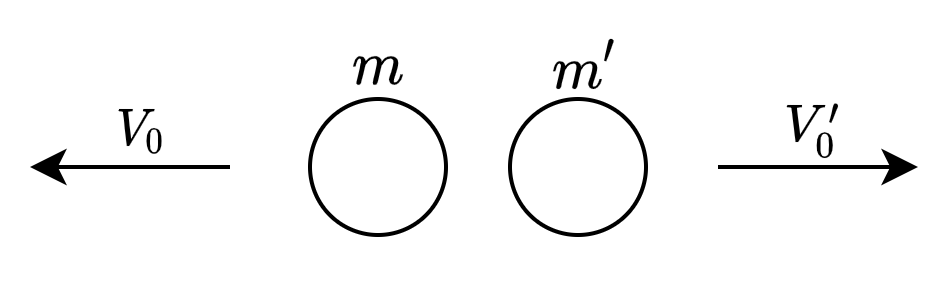
\includegraphics[width=0.6\textwidth]{Percussion1D3-Apres.png}}
    \caption{Situation après contact 1D.}
    \label{fig:contact1dapres}
\end{figure}

\noindent On obtient l'\cref{eq:crammer2}:
\begin{align} \label{eq:crammer2}
    - V_0 + V'_0 = \varepsilon (v_0 - v'_0) \,.
\end{align}
Le système de Cramer qui découle des \cref{eq:crammer1,eq:crammer2} permet d'obtenir les expressions:
\begin{align} \label{eq:vitessesapres1D}
    V_0 = \frac{I + (m-\varepsilon m')v_0 + (1+\varepsilon)m'v'_0}{m+m'} \,, \quad V'_0 = \frac{I + (1+\varepsilon)mv_0 + (m'-\varepsilon m)v'_0}{m+m'}\,.
\end{align}

% Nous faisons donc ici la grosse hypothèse que \underline{le mouvement de $x_2$ et $x_3$ devient uniforme après la collision}. 

Une fois leur vitesses "initiales"\footnote{Ces vitesses sont les vitesses de départ pour le deuxième phase de la percussion.} obtenues, on calcule donc les déplacements des différents noeuds des réseaux, et les fractures éventuelles qui s'en suivent. Plus précisément, on a par exmple pour le premier floe:
\begin{itemize}
    \item son noeud de gauche $x_1$ a pour vitesse $v_0$ avant et le choc et conserve cette vitesse après le choc;
    \item son noeud de droite $x_2$ a pour vitesse $v_0$ avant le choc, mais passe de facon discontinue à $V_0$ apres le choc.
\end{itemize}
En procédant de manière similaire, nous obtenons les déplacements et les vitesses des noeuds du deuxième floe après la collision. Une simulation permet d'obtenir le résultat de la \cref{fig:frac1d3}.
\begin{figure}[!h]
    \centering
    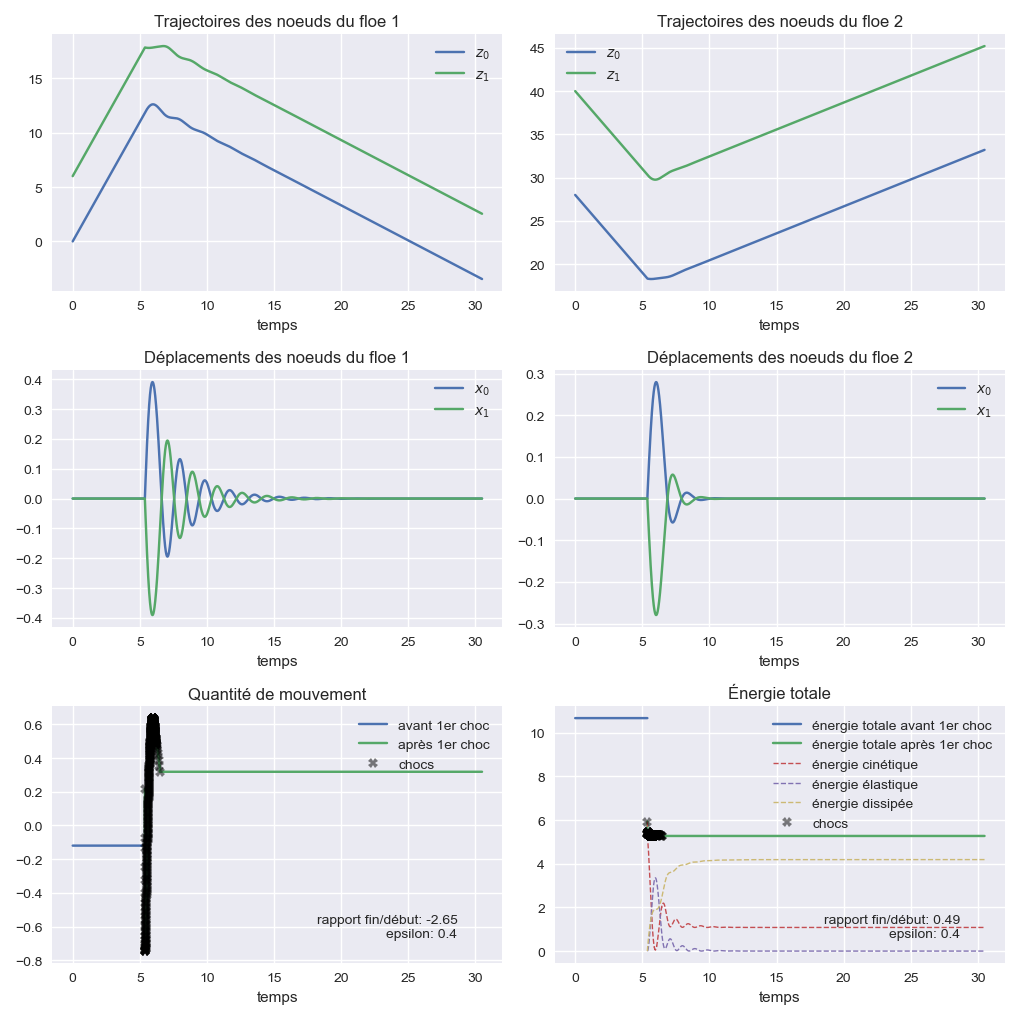
\includegraphics[width=0.8\textwidth]{EnsPlotPerc1.png}
    \caption{Un résultats obtenus avec le premier modèle pour la percussion avec trois floes. Les paramètres de ce problème peuvent etre récupéres dans le dépot GitHub (voir \href{https://github.com/desmond-rn/ice-floes/blob/master/code/simu1D/PercussionSolver.py}{PercussionSolver.py}), et la simulation correspondante à travers ce LIEN SEAFILE.}
    \label{fig:frac1d3}
\end{figure}

% N'ayant aucune garantie que les vecteurs vitesses $v_0$ et $V_0$ seront opposés immédiatemetn après le choc, nous ne pouvons garantir la convergence de ce modèle (voir \cref{th:div1D}). Ce modèle dégénère (probablement) après la première collision. Effectuons à présent une modélisation 2D et observons si le même problème se repète.

%%-------Pas vrai
% Pour $\varepsilon \neq 0$, l'\cref{eq:crammer2} permet de constater que $V_0 = V'_0$ si et seulement si $v_0 = v'_0$. En se basant sur le \cref{th:div1D}, nous pouvons donc énoncer le corrolaire suivant:

% \begin{corollary} \label{cr:div1D}
%     Le modèle de collision inélastique 1D avec séparation des masses converge si les vitesses des noeuds avant le choc sont des vecteurs opposés.

%     Le modèle de collision inélastique 1D avec séparation des masses converge si et seulement si leurs vitesses initiales sont des vecteurs opposés.
% \end{corollary}
% \begin{proof}
%     La preuve découle immédiatement du \cref{th:div1D}.
% \end{proof}

% \noindent Le \cref{cr:div1D} permet de constater les limites de notre modélisation 1D. En effet, les moceaux de glace dans la MIZ ne dérivent pas tous à la meme vitesse. Effectuons à présent une modélisation 2D et observons si le même problème se repète.





\subsection{Deuxième modèle pour la collision avec séparation des masses}
\label{subsec:model1d2}



Dans cette section, nous introduisons un modèle 1D plus général que ceux présentés dans les deux sections précédentes (voir \cref{subsubsec:moddep1D,subsubsec:colinesepma}). Les floes sont cette fois représntés par une multitude de noeuds, de ressorts et de dispositifs visqueux. 
\begin{figure}[!h]
    \centering
    \frame{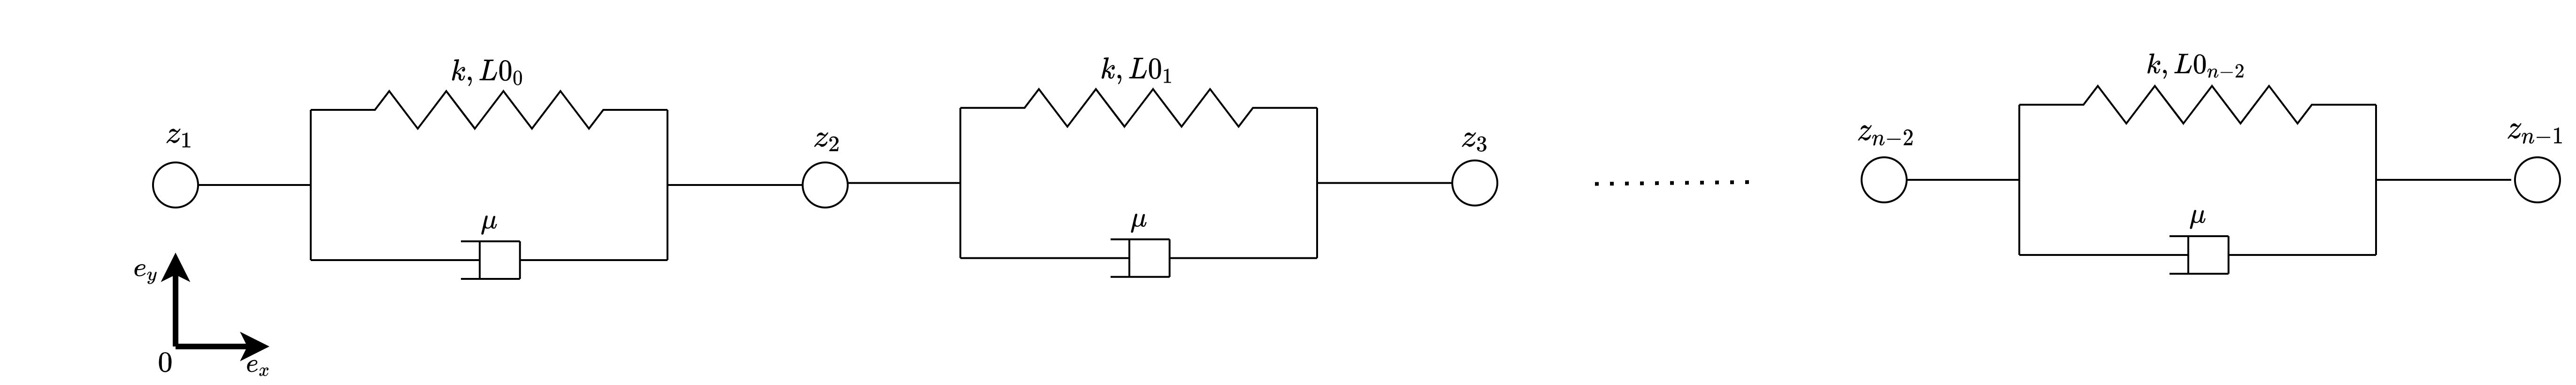
\includegraphics[width=0.8\textwidth]{Deplacement1D-2.png}}
    \caption{Modélisation d'un floe 1D comme un assemblage de $n$ masses reliées par des ressorts et des dispositifs visqueux. Nous nous servons dorénavant des positions $z$ des neouds dans le repère absolu. $k$ est la constante de raideur uniforme de tous ses ressorts, et $\mu$ le coefficient de dissipation pour tous les dispositifs visqueux. Aussi, le terme $L0_i$ désigne les longueur à vide du ressort $i$.}
    \label{fig:dep1d4}
\end{figure}
Contrairement à l'approche par déplacement que nous avons adopté à la \cref{subsubsec:moddep1D}, nous considérons ici une approche par position des noeuds dans le repère absolu $\mathcal{R}= (O, \bvec{e}_x, \bvec{e}_y)$ (voir \cref{fig:dep1d4}).\footnote{Pour une raison inexpliquée, l'approche par déplacement ici ne conserve pas les positions à l'équilibres des ressorts.} Signalons que dans la suite, les dispositifs visqueux ne serons plus représenté afin de faciliter les simulations.  

Commencons par simuler les déplacements et les vitesses des noeuds d'un floe contenant $n$ noeuds. De facons similaire aux sections précédentes, la loi de comportement du système est la suivante:
\begin{align} \label{eq:multiressortsdep}
    \begin{dcases}
        m\ddot z_0 = k(z_1 - z_0 - L0_0) + \mu (\dot z_1 - \dot z_0)\, , \\
        m\ddot z_1 =  k(z_2 - z_1 - L0_1) + \mu (\dot z_2 - \dot z_1) - k(z_1 - z_0 - L0_0) - \mu (\dot z_1 - \dot z_0) \,, \\
        \qquad \vdots \\
        m\ddot z_{n-1} = k(z_{n-1} - z_{n-1} - L0_{n-2}) + \mu (\dot z_{n} - \dot z_{n-1}). 
    \end{dcases}
\end{align}
Pour résoudre ce système, nous le posons sous forme matricielle, et nous le transformons en un système d'EDO du premier ordre. On obtient:
\begin{align} \label{eq:percussion1d4}
    \begin{pmatrix}
        \dot z_0 \\ \dot z_1 \\ \vdots \\ \dot z_{n-1} \\ \ddot z_0 \\ \ddot z_1 \\ \vdots \\ \ddot z_{n-1}
    \end{pmatrix}
    = 
    \underbrace{\begin{pmatrix}
        \begin{matrix}
       & & &  \\ & & &  \\ & & \bigzero & \\ & & & \\      
        \end{matrix}
        & \rvline 
        & \begin{matrix}
        & & & \\ & & &  \\ & & I_n & \\ & & & \\
        \end{matrix}  \\ 
        \hline
        \begin{matrix}
            & & &  \\ & & B & \\ & & & \\ & & & \\     
        \end{matrix}
        & \rvline 
        &\begin{matrix}
            & & & \\ & & C & \\ & & & \\ & & & \\        
        \end{matrix}
      \end{pmatrix}}_{2n \times 2n}
      \begin{pmatrix}
        z_0 \\ z_1 \\ \vdots \\ z_{n-1} \\ \dot z_0 \\ \dot z_1 \\ \vdots \\ \dot z_{n-1}
        \end{pmatrix}
    +
    \underbrace{\begin{pmatrix}
        \begin{matrix}
       & & &  \\ & & &  \\ & & \bigzero & \\ & & & \\      
        \end{matrix}
        & \rvline 
        &     \begin{matrix}
            & & &  \\ & & &  \\ & & \bigzero & \\ & & & \\      
             \end{matrix}  \\ 
        \hline
        \begin{matrix}
            & & &  \\ & & D & \\ & & & \\ & & & \\     
        \end{matrix}
        & \rvline 
        &   \begin{matrix}
            & & &  \\ & & \bigzero &  \\ & &  & \\ & & & \\      
            \end{matrix}
      \end{pmatrix}}_{(2n) \times (2n-2)}
      \begin{pmatrix}
        L0_0 \\ L0_1 \\ \vdots \\ L0_{n-2} \\ 0 \\ 0 \\ \vdots \\ 0
        \end{pmatrix} \,,
\end{align}
où $I_n$ est la matrice identité de taille $n$; $B$ et $C$ des matrices de taille $n\times n$; et $D$ une matrice de taille $(n) \times (n-1)$. On a:
$$
B = \frac{1}{m} \begin{pmatrix}
    -k & k &  &  &  \\
    k & -2k & k &  &  \\
     & \ddots & \ddots & \ddots &  \\
     &  & k & -2k & k \\
     &  &  & k & -k
    \end{pmatrix} \, , \quad 
C = \frac{1}{m} \begin{pmatrix}
    -\mu & \mu &  &  &  \\
    \mu & -2\mu & \mu &  &  \\
     & \ddots & \ddots & \ddots &  \\
     &  & \mu & -2\mu & \mu \\
     &  &  & \mu & -\mu
    \end{pmatrix} \, , \text{ et}\quad 
D = \frac{1}{m} \begin{pmatrix}
    -k &  &  &  \\
    k & -k &  &  \\
     & \ddots & \ddots &  \\
     &  & \ddots & -k \\
     &  &  & k 
    \end{pmatrix}\,.
$$

Concernant la percussion\footnote{Tout comme dans les sections précédentes, nous réservons l'exposant "prime" (') pour décrire les paramètres du deuxième floe de glace.}, nous proposons aussi une approche différente de calculer les vitesses des noeuds après choc. En effet, nous appliquons non pas le principe de la conservation de la quantité de mouvement, mais celui de la conservation de l'énergie cinétique. Ce choix provient du fait que dans ce modèle, les deux noeuds en contact ne sont pas considérés comme un système isolé. En effet, les deux noeuds sont affectés par les forces des ressorts et des dispositifs visqueux qui leur sont ratachés. Ces deux forces ont un travail non nul et ne sont donc pas conservatives (voir \cref{fig:situationcontact4}). 
\begin{figure}[!h]
    \begin{subfigure}[b]{0.48\textwidth}
        \centering
        \frame{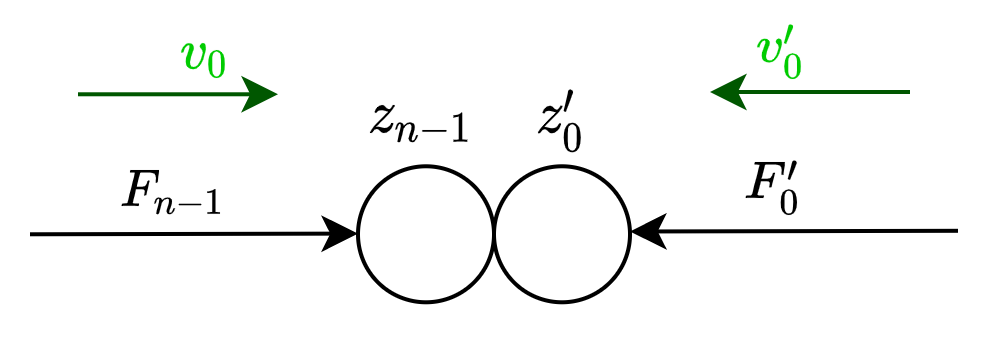
\includegraphics[width=\textwidth]{Percussion1D-4-Avant.png}}
        \caption{Avant le choc}
    \end{subfigure}
%     \hfill
    \begin{subfigure}[b]{0.48\textwidth}
        \centering
        \frame{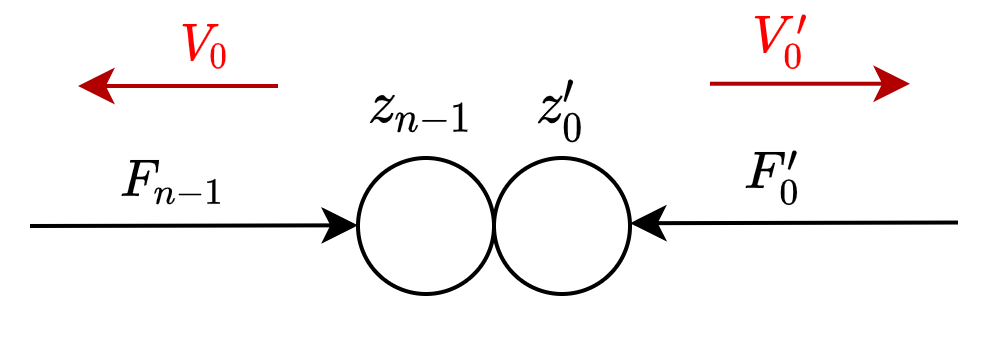
\includegraphics[width=\textwidth]{Percussion1D-4-Apres.png}}
        \caption{Après le choc}
    \end{subfigure}
       \caption{Situation avant et après la percussion de deux floes. Nous considetons ici que le floe de gauche dans la percussion possède $n$ noeuds. Les forces appliquées par les floes voisins aux noeuds en contact sont: $F_{n-1} = k(z_{n-1} - z_{n-1} - L0_{n-2}) + \mu (\dot z_{n} - \dot z_{n-1})$, et $F'_0 = k'(z'_1 - z'_0 - L0'_0) + \mu (\dot z'_1 - \dot z'_0)$, conformément à l'\cref{eq:multiressortsdep}.}
       \label{fig:situationcontact4}
\end{figure}
Nous appliquons donc la conservation de l'énergie cinétique pour obtenir une équation pour les vitesses après choc:
\begin{align}
    \frac{1}{2}m v_0^2 + \frac{1}{2}m' (v'_0)^2 = \frac{1}{2}m V_0^2 + \frac{1}{2}m' (V'_0)^2\,.
\end{align}
Nous maintenons l'équation de restitution \cref{eq:crammer2} utilisé dans les sections précédentes:
\begin{align}
    - V_0 + V'_0 = \varepsilon (v_0 - v'_0) \,.
\end{align}
La résolution du système ci-haut nous permet d'obtenir les vitesses $V_0$ et $V'_0$ respectivement pour les noeuds de gauche et de droite dans la collision\footnote{Notons que les tous les noeuds qui ne sont pas en contact conservent leurs vitesss pendant le choc.}.:
\begin{align}
V_0 = \frac{-b \pm \sqrt{\Delta}}{2a}, \text{ et} \quad V'_0 = V_0 + X\,,
\end{align}
avec :
$$
X= \varepsilon(v_0 - v'_0), Y = m(v_0)^2 + m'(v'_0)^2,  a = m+m', b = -2m'X, c = m'X^2 - Y, \text{ et } \Delta = b^2 - 4ac.
$$


Pour tester ce modèle, nous effectuons des simulations avec trois noeuds ayant $7$ et $8$ neuods respectivement. Nous étudions aussi la conservation de la quantité de mouvement et de l'énergie mécanique totale\footnote{Somme de l'énergie cinétique, de l'énergie potentielle élastique, et de l'énergie dissipée par frotement visqueux.} et nous obtenons les résultats présentés à la \cref{fig:frac1d4}.
\begin{figure}[!h]
    \centering
    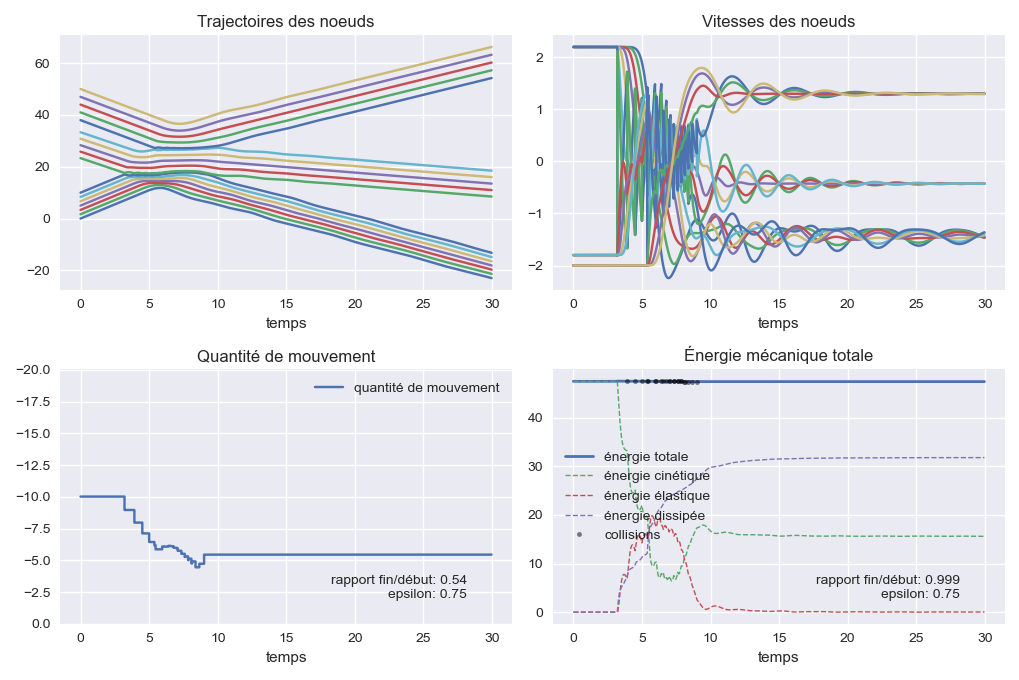
\includegraphics[width=0.85\textwidth]{EnsPlotPerc2.png}
    \caption{Un résultats obtenus avec le deuxième modèle pour la percussion avec trois floes. Les paramètres de ce problème peuvent etre récupéres dans le dépot GitHub (voir \href{https://github.com/desmond-rn/ice-floes/blob/master/code/simu1D/FractureSolver.py}{FractureSolver.py}), et la simulation correspondante à travers ce LIEN SEAFILE.}
    \label{fig:frac1d4}
\end{figure}
Bien que ce modèle conserve l'énergie mécanique du système (voir \cref{fig:frac1d4}), nous nous rendons compte qu'il présente plusieurs manquements; en particulier que la conservation de l'énrgie cinétique entre en opposition directe avec la notion d'élastitité au rebondissement (traduite par le coeffient de restitution $\varepsilon$). C'est pour résoudre ces problèmes que nous avons développé un troisième modèle pour la percussion 1D.





\subsection{Troisième modèle pour la collision avec séparation des masses}
\label{subsubsec:troisiemecol}

Ce modèle a été développé pour aborder la question de non conservation de l'énergie mécanique totale après la collision.
Il prend plus au sérieux la question du passage macro/micro. Celà dit, les équations qui régissent le déplacement des noeuds (voir EQUATION ...) de chaque floe en collision sont maintenues. La différence avec le modèle présenté dans la sous-section précédente (\cref{subsec:model1d2}) apparait au niveau du calcul des vitesses après choc.

Rappelons que le modèle macroscopique a été développé par M. Rabatel, S. Labbé, et J. Weiss \parencite{rabatel2015dynamics} et nous l'avons présenté avec détails à travers un résumé de la thèse de M. Rabatel \parencite{rabatel2015thesis} dans la \cref{sec:thesematthias}. Le modèle qui y est développé considère un morceau de glace comme un solide indéformable et le système perd de l'énergie mécanique à travers le coefficient de restitution macroscopique $\varepsilon$. Dans le modèle miscroscopique que développons ici, les floes sont des solides élastiques (système masse-ressort-dispositif visqueux) et le problème est de trouver à quelle perte d'énergie le $\varepsilon$ correpondrait lorsque deux noeuds de deux floes entrent en collision. Autrement dit, il faudrait trouver une correspondance entre les coefiencents de restitution macoscopiques et microscopiques.

Notre système de deux noeuds au moment de la collision perd donc de l'énergie. L'absence de forces de frotements\footnote{Dans le modèle actuel, les frotements de l'air et de la mer ne sont pas pris en compte.} veut dire que l'énergie mécanique est transformée en énergie interne (thermique). 
\begin{figure}[!h]
    \centering
    \frame{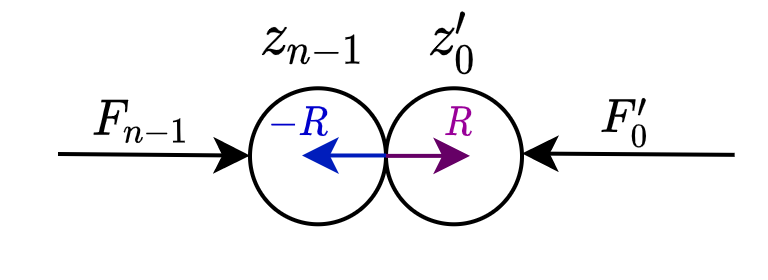
\includegraphics[width=0.6\textwidth]{Percussion1D-5.png}}
    \caption{Situation durant la percussion de deux floes. Nous observons ici la force $R$ exercée par chaque noeud sur l'autre, qui sui la loi de l'action et de la réaction.}
    \label{fig:situationcontact5}
\end{figure}
Les \cref{fig:situationcontact4,fig:situationcontact5} permettent de mieux appréhender la percussion dans ce cas. Pour calculer les vitesses des noeuds après choc, nous reconsidérons \cref{eq:crammer2} qui introduit le coefficient de restitution de Newton:
\begin{align} \label{eq:perc5eq1}
    V_0 - V'_0 = - \varepsilon (v_0 - v'_0) \,.
\end{align}
Pour trouver une deuxième équation et obtenir les vitesses des noeuds, nous nous tournons vers une technique fréqument utilisée dans l'industrie du jeux vidéo\parencite{hecker1997collision} pour gérer les collisions d'objets. Dans cette technique, nous considérons que la collision se produit entre les instants $t^{-}$ et $t^{+}$. Cet intervalle de temps, très cours, fut calculé durant les travaux de M. Rabatel \parencite[p.87]{rabatel2015thesis} sur la collusion rigide entre deux floes. On a:
$$
m \ddot z_{n-1} = F_{n-1} - R, \text{ et} \quad  m'z'_0 = F'_0 + R.
$$
Après avoir intégré ces équations tout en supposant que les forces $F_{n-1}$ et $F'_0$ restent constantes\footnote{En effet, la durée de la percussion est négligeable à l'échelle des temps de simulation.} entre $t^{-}$ et $t^{+}$, nous posons:
$$
I = \int_{t^{-}}^{t^{+}} R \diff t, \quad  J = \int_{t^{-}}^{t^{+}} F_{n-1} \diff t = F_{n-1} \Delta t, \text{ et} \quad  K = \int_{t^{-}}^{t^{+}} F'_{0} \diff t = F'_{0} \Delta t.
$$
On obtient donc deux équations supplémentaires pour former le système d'\cref{eq:perc5eq1,eq:perc5eq2,eq:perc5eq3}.
\begin{align} \label{eq:perc5eq2}
    V_0 = v_0 + \frac{J-I}{m} \,,
\end{align}
\begin{align} \label{eq:perc5eq3}
    V'_0 = v'_0 + \frac{K+I}{m'}.
\end{align}
Le calcul de la quantité $I$ permet donc d'achever la résolution de ce système. A cet effet, nous obtenons:
\begin{align}
    I = \frac{(v_0 - v'_0)(1+\varepsilon) +\frac{J}{m} - \frac{K}{m'}}{\frac{1}{m}+\frac{1}{m'}}
\end{align}

Pour tester ce modèle, nous avons éffectué la mêmes simulation qu'avec le modèle précédent. Rappellons que la seule différence entre ces deux modèle est le tratement des vitesses après contact. Les résultats sont donc résumés à la FIGURE CI-BAS:
\begin{figure}[!h]
    \centering
    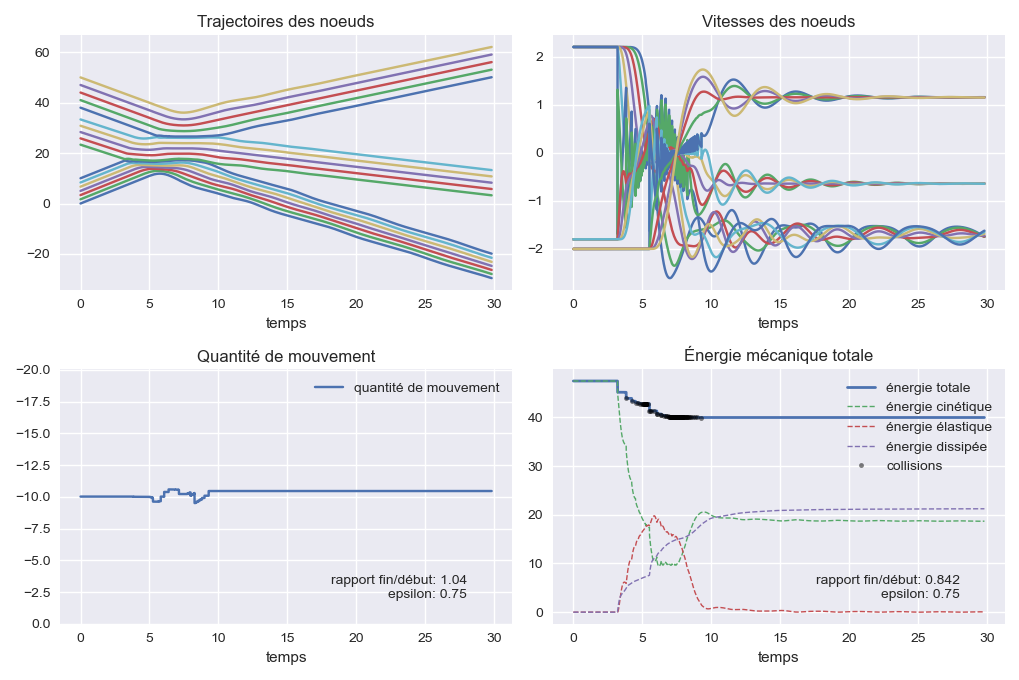
\includegraphics[width=0.85\textwidth]{EnsPlotPerc3.png}
    \caption{Un résultats obtenus avec le troisième modèle pour la percussion avec trois floes. Les paramètres de ce problème peuvent etre récupéres dans le dépot GitHub (voir \href{https://github.com/desmond-rn/ice-floes/blob/master/code/simu1D/FractureSolver.py}{FractureSolver.py}), et la simulation correspondante à travers ce LIEN SEAFILE.}
    \label{fig:frac1d5}
\end{figure}

Nous obervons effectivement qu'il y a diminution de l'énergie totale à chaque collision. Cependant, il reste à savoir si cette perte d'énergie au niveau microscopique correspond à la perte observée au niveau macroscopique (passage micro/macro), surtout lorsque surviennent des fractures dans les floes.


%3----------------------------------------------------------------------------------------





\section{Modélisation de la fracture}


\subsection{Méthode du champ de phase}
\label{subsubsec:approchephase}

La nécésité de prédire les fractures des matériaux dans les matériaux industriels gagne en importance chaque année. En méchanique des sciences computationnelles, la Virtual Crack Closure Technique (VCCT) (REFERENCE A LA PAGE 2 DE PHASE FIELD EN ANGLAIS), la Extended Finite Element Method (X-FEM), Cohesive Zone Method (CZM), et d'autres models de fractures discret représentent la fracture comme une entité discontinue à partir de laquelle la variable d'intéret est obtenue. Ces méthodes demandent non seulement des re-maillaiges plus fins, mais aussi des algorithms robustes pour pouvoir capturer les fractures. Ceci est numériquement couteux, particulèrement lorsque les fractures ont des géoétries complexes.

FIGURES (a) et (c) de FIGURE 1 DU PHASE FIELD EN FRANCAIS

L'approche par champ de phase est née des travaux de Franckfort et Marigo (REFERENCE), et de leur régularisation par Bourdin de al. (REF). Rappellons que l’approche variationnelle développée dans ces travaux consiste à formuler le problème de fissuration comme un problème de minimisation de l’énergie du solide fissuré exprimée comme:

ÉQUATION 1 DE PHASE FIELD EN FRANCAIS

Cette approche conduit à une implémentation numérique élégante où les complexité dues aux fractures discrètes sont élimiées. Pour éviter cette difficulté, une approche régularisée de la description
des discontinuités associées aux fissures consiste à remplacer la fonctionnelle originale par une fonctionnelle approchée (REFERENCES PHASE FIELD EN FRANCAIS). Dans ce cadre, les fissures ne sont plus décrites par des surfaces mais par un champ de phase endommagée $d(\bvec{x})$. L’énergie est alors exprimée par:

ÉQUATION 2 DE PHASE FIELD EN FRANCAIS

En introduisant une discrétisation en temps $T = \{ t^0, t^1, \ldots, t^n, t^{n+1}, \ldots, t^N \}$. A chaque pas de temps $t^{n+1}$, le problème consiste à déterminer le champ de déplacements $u^{n+1}$ et le champ de phase endommagée $d^{n+1}$ tels que :
$$
\bvec{u}^n+1, d^{n+1} = \underset{\bvec{u}\in \mathcal{K}_A \\ 0 \leq d^n \leq d^{n+1}}{argmin} E
$$
où $\mathcal{K}_A$ est un champ de déplacements cinématiquement admissible. Un exemple de densité de fissure pour un modèle de premier ordre est donné par :
$$
\gamma (d, \nabla d) = \frac{1}{2l}d^2 + \frac{l}{2}\nabla d \cdot \nabla d,
$$
où $l$ est un paramètre de régularisation des discontinuités de fissures. Une fonction d'histoire est introduite pour décrires les effets d'histoire, et des possibles chargments et déchargements \parencite{miehe2010phase}:
\begin{align}
    \label{eq:histoire}
    \mathcal{H}(\bvec{x}, t) = \max{\Psi^{+}(\bvec{x},\tau)}_{\tau \in [0,t]} .
\end{align}
Dans \cref{eq:histoire}, $\Psi^+$ est la partie positive de la fonction densité d’énergie élastique telle que $\Psi(\varepsilon) = \Psi^{+}(\varepsilon) + \Psi^{-}(\varepsilon)$
et est définie par :

EQUATION 8

où $\varepsilon$ est le tenseur des déformations linéarisé. $\langle x\rangle_{\pm} = (x \pm \vert x \vert) / 2$ et $\varepsilon^{\pm}$ sont les parties positives et négatives du tenseur des déformations. Nous posont à présent $g_c$ le taux de liération critique de l'énergie de type Griffith \parencite[p.5]{miehe2010phase}, $\bvec{f}$ un vecteur de forces de volumes, $\bar{u}$ et $\bar{F}$ les déplacements et efforts imposés sur les bords associés $\partial \Omega_u$ et $\partial \Omega_F$ (VOIR FIGURE CI-HAUT). Nous écrivons enfin la loi de comportement comme:

EQUATION 9

ce qui nous permet d'obtenir le probèleme couplé suivant pour déterminer $d(\bvec{x})$ et $\bvec{u}(\bvec{x})$.

EQUATIONS 5 ET 6


Quelques résultats obtenus par cette méthode ont été présentés dans les travaux de D. Balasoiu à la SECTION (VOIR FIGURE). Malgrès l'éfficacité de cette méthode, notre travail à son sujet durant ce stage s'est limité à son assimilation. En effet, nous ne l'avons pas implémentée par faute de temps. Il se trouve qu'en 1D avec un fable nombre de noeuds, une astuce alternative est envisageable. 




\subsection{Une approache combinatoire pour la fracture}
\label{subsubsec:approchecombi}


Etant donné le déplacement des noeuds du floes à un temps précis $t^{n+1}$, nous recherchons la fracture qui minimise l'énergie potentielle totalle au temps $t^{n+1}$:
\begin{align}
    \boxed{
    \begin{array}{rcl}
    E^{n+1} & = \text{énergie potentielle élastique au temps } t^{n+1}  \\
    & + \text{ténacité}\times \text{longeur de la fracture évenetuelle au temps }t^{n+1}.  
    \end{array}
    }
\end{align}
La longeur de la fracture correspondant ici à la longueur à vide du ressort\footnote{Nous utiliserons la désignation \emph{ressort} ici pour indiquer à la fois le ressort et le dispositif visqueux situé entre deux neouds adjacents (VOIR FIGURE SUR LA PARTIE PRÉCÉDENTE)} à cette position si celui ci s'était brisé. Notre approche combinatoire consite ainsi à calculer les énergie correspond à toutes les fractures possibles dans le floe, et nous récupérons la plus petite de ces énergies $E^{n+1}_{min}$. Conformément à l'approche de Griffith, une fracture n'apparait que si $E^{n+1}_{min}\leq E^{n}_{min}$.

FIGURE ILLUSTRATIVE DE CETTE APPROCHE


L'approche combinatoire n'est supportable qu'en 1D car à chaque pas de temps, il y a autant de fracture admissibles qu'il ya de ressorts\footnote{En réalité, les deux ressorts exptrèmes ne peuvent se briser, car cela donnerait naissance à des floes sans ressorts}. En effet, à chaque ressort brisé, c'est un nouveau floe qui est créé. Cette simplication élimine aussi le problème de \emph{propagation de la fracture}; en 1D, nous ne traiterons donc que le problème de \emph{nucléation de la fracture}. 

Tous ceci n'est évidement pas le cas en dimension supérieur, et nous devons étudier toutes les combinaisons psossibles de ressorts qui cèdent simultanément; ce qui est très couteux. Il est donc primordial d'implémenter la méthode du champ de phase pour toute adaptation de nos résultats en dimension 2 ou 3.


%4----------------------------------------------------------------------------------------





\section{Algorithme de calcul 1D}


Nous présentons dans cette section l'algorithme que nous avons adopté pour développer notre code de simulation de la percussion ainsi que la fracture de floes 1D. Notons que l'implémtation de la percussion correspond au modèle présenté à la \cref{subsubsec:troisiemecol}. Cependant, les autres modèles de percussion peuvent facilement etre obtenus en changeant le contenu de la fonction \texttt{computeAtContact} que nous détaillerons plus tard. Quant à la fracture, nous avons implémenter l'approche combinatoire présentée à la \cref{subsubsec:approchecombi}. En résumé, l'algorithme dans l'intervalle de temps $[t^n, t^{N}]$ est le suivant:

METTRE L'ALGORITHME DANS UNE BOITE
\begin{enumerate}
    \item Initialisation: Les positions $\bvec{q}^{n}$, les vitesses $\bvec{v}^n$ de tous les noeuds de tous les floes sont connus. Mettre à jours les chargements aux bords au temps courant $t^{n+1}$\footnote{Pour simplifier nos calculs, aucun chargement n'est imposé aux bords du floe; nous avons des conditions de Neumann durant toutes nos simulations.}
    \item Calcul des déplacements: Calcul des postions des noeuds $\bvec{q}^{n+1}, \ldots \bvec{q}^{N}$ et des vitesses associées $\bvec{v}^{n+1}, \ldots \bvec{v}^{N}$. Nous utilisont ici les équations ... 
    \item Détection des fractures: pour chaque pas de temps $t^k \in [t^{n+1}, t^{N}]$ et pour chaque floe, rechercher la configuration qui présente l'énergie potentielle totale minimale $E^{k}_{min}$, et la comparer avec l'énergie $E^n_{min}$. En cas de fracture, i.e. $E^{k}_{min} \leq E^n_{min}$, on retient l'indice de fracture potentielle\footnote{Les indices potentielles sont aussi les temps à partir desquels nous vérifions les fractures/collisons à l'étape suivante} du floe concerné (disons $f$) $\text{checkFrac}_f = k$; sinon, $\text{checkFrac}_f = N$.
    \item Détection des collisions: pour chaque pas de temps $t^k \in [t^{n+1}, t^{N}]$ et pour chaque noeud, on se demande s'il y a collision avec le noeud voisin de droite. En cas de collision,, on retient l'indice de collision potentielle des noeuds concerné (disons $e_1$ et $e_2$) $\text{checkColl}_{e_1} = \text{checkColl}_{e_2} =k$; sinon, $\text{checkColl}_{e_1} = \text{checkColl}_{e_2} = N$.
    \item Mise à jour des indices potentielles de fracture: Tous ces indices sont reinitialisés au minimum de tous les indices de fracture $\text{checkFrac} = \min{\text{checkFrac}_f}_{f \in \mathcal{F}}$, où $\mathcal{F}$ désigne l'ensemble des floes.
    \item Mise à jour des indices potentielles de collision: Désignons par $\text{checkColl}'$ le minimum de tous les indices de collisions$\min{\text{checkColl}_e}_{e \in \mathcal{E}}$, où $\mathcal{E}$ désigne l'ensemble des neouds du problème. Tous les indices sont reinitialisés à $\text{checkColl} = \min{\text{checkColl}', \text{checkFrac}}$.
    \item Invalidation des quantités: Toutes les positions et les vitesses calculées (à l'étape $2$) qui survienne après une collision ou une fracture sont invalidées.
    \item Finalisation: on recommence à l'étape $1$ à partir de $\text{checkColl}$. On repète ainsi jusqu'a ce que $\text{checkColl} = N$
\end{enumerate}


Notons que l'algorithme présenté ci-haut omet plusieurs détails indispensables pour une implémentation efficace en language Python. Par exemple, l'invalidation des quantitées est prise en main par les fonctions de détection des collision et de fracture. Nous fournissons donc la méthode $\texttt{runSimulation()}$ de la classe $\texttt{FractureSolver}$ ci-bas:

COLLER COLLER runSimulation (Indiquer ce que chaqune des fonction indiquée fait)

Pour mieux assimiler le programme, nous proposons ci-bas un diagramme UML qui illustre la structure du code à travers ses différentes classes et fonctions.

DIAGRAMME UML ET README DU REPOSITORY (Indiquer qu'il suffit de changer la fonction computeAtContact pour passer d'un modèle à l'autre.)

Tous ce code est stocké dans un dépot GitHub privé dont une explication du contenu est donnée dans le fichier README dont la capture est présentée ci-bas. 

README DU REPO GITHUB


Nous fournissons aussi ci-bas quelques frames d'un simulation obtenue par le l'algorithme et le code Python présentés ci-haut:

PRÉSENTER 5 A 10 TIME STEPS D'UNE SIMULATION AVEC PLUSIEURS FLOES


%4----------------------------------------------------------------------------------------

\section{Résumé des résultats obtenus}


Pour le problème 1D, nous avons non seulemetn étudié le déplacement des noeuds d'un floe, mais aussi ce qui se passe après une collision de ces noeuds. En considérant le floe comme un réseau de ressorts, nous avons pu étudier la nucléation (et la propagation) d'une fracture suivant le modèle de Griffith sans recourir à la méthode du champ de phase.

Nous avons éffectué plusieurs simulation qui ont montrer que les ressorts se brisent lorsqu'ils sont fortement compréssés. Le modèle 1D adopté (voir \cref{subsubsec:troisiemecol}) a également montré que le système perds de son énergie (cinétique) au cours du temps, ce qui 


Quand à la validation des résultats, nous n'avons pas réussi à effectuer des tests en laboratoire. Cette tache représente la prochaine étape avant l'adoption de ce modèle 1D. Ceci dit, les floes de glace sont généralement considérés comme des objets 2D du fait de leur taille négligeable face au rayon de la terre. Une étude en dimension supérieure est donc indispendable pour un déployment de notre modèle de fracture à l'échelle des floes de glace.










